\chapter{Newtonian Mechanics}
Newtonian mechanics is the framework, derived by Isaac Newton in $1687$, the describes physics of point particles in the non-relativistic, macroscopic limit (i.e. the limit in which the effect of relativity and quantum mechanics can be neglected). The centerpiece of Newtonian mechanics is Newtons five laws and the laws, the principle of conserved quantities and the choice of reference frame.


\section{Newtons laws}
\index{Newtons laws}
Armed with the enormous empirical material which is condensed in the laws of Kepler and Galileo, Isaac Newton managed to discover his famous laws of motion alongside the law of gravitational interaction. Newtons five laws of motion can be stated as follows~\citep{hjort}
\begin{enumerate}
	\item \emph{The law of inertia:} A body which is not acted upon by any force will either be at rest or in a state of uniform,  linear motion. This law is manifested in the definition of linear momentum. The linear momentum of an object is defined as the mass of the object, $m$, times the velocity of the object, $\vec{v}$, i.e.
	\begin{equation}
		\vec{p}=m\vec{v}=m\dot{\vec{x}},
	\end{equation} 
	where the dot indicates the time derivative of the position vector. From the definition of linear momentum, the law of inertia can be stated as follows
	\begin{equation}
		\text{No external force} \Rightarrow \vec{p}= \text{constant vector}.
	\end{equation} 
	In this way the law of inertia coincides with the law of conservation of linear momentum for an isolated particle. 
	
	\item \emph{The law of acceleration:} The mass, $m$, of a body, times its acceleration, $\vec{a}$, equals the force, $\vec{F}$, on the body, i.e. 
	\begin{equation}
		\vec{F}=m\vec{a}=m\ddot{\vec{x}},
	\end{equation} 
	where the dots denote the second time-derivative of the position vector. From the definition of linear momentum, the law of acceleration can be written as follows
	\begin{equation}
		\vec{F}=\frac{d\vec{p}}{dt}.
	\end{equation} 
	
	\item \emph{The law of action and reaction:} If body A acts on body B with a force, then body B will act on body A with an equal but oppositely directed force.
	
	\item \emph{The postulate of absolute time:} Absolute, true, and mathematical time, of itself, and from its own nature, flows equally without relation to anything external, and by another name is called duration.
	
	\item \emph{The postulate of absolute space:} Absolute space, in its own nature, without relation to anything external, remains always similar and immovable.
\end{enumerate} 
The five laws are, in the form stated above, only valid in what is called an inertial reference frame. An inertial reference frame is defined as a reference frame in which Newtons first law (the law of inertia) holds true. That is to say an inertial reference frame is a reference frame in which if an object is not subject to a resulting force, it will remain at rest or move with a uniform velocity, i.e. it will not accelerate. A non-inertial reference frame is a reference frame in which Newtons first law does not hold. Examples of non-inertial reference frames are eg. rotating reference frames or accelerating reference frames. The reader may be familiar with riding a marry-go-round or accelerating in a car. In both cases the reader might recall being pushed outwards or back into th seat. In both cases, the body is required to either hold onto the marry-go-round or push back into the seat, in order to remain at rest in the car or the marry-go-round. Hence, both of these reference frame are not inertial.
\begin{example}
	An important example of a force is the gravitational force in the Newtonian limit. Newtonian gravity states that the gravitational force between two particles act to attract the two particles. The force is given by
	\begin{equation}
		\vec{F}_g=-\frac{G_Nm_1m_2}{r^2}\hat{r}=m_1\vec{g},
	\end{equation} 
	where $G_N=6.67\cdot 10^{-11}\frac{Nm^2}{kg^2}$ is Newtons gravitational constant, $m_i$ are the masses of the two particles and $r$ is the radial vector connecting the two particles. The minus sign indicated the force is attractive.
\end{example}
\begin{example}
	\emph{Determine and solve the EOM for a simple pendulum.}\newline
	
	The simple pendulum is a mass hanging from a massless string, free to swing (see figure \ref{fig:pen}).
	\begin{figure}[H]
		\captionsetup{width=1\textwidth}
		\centering
		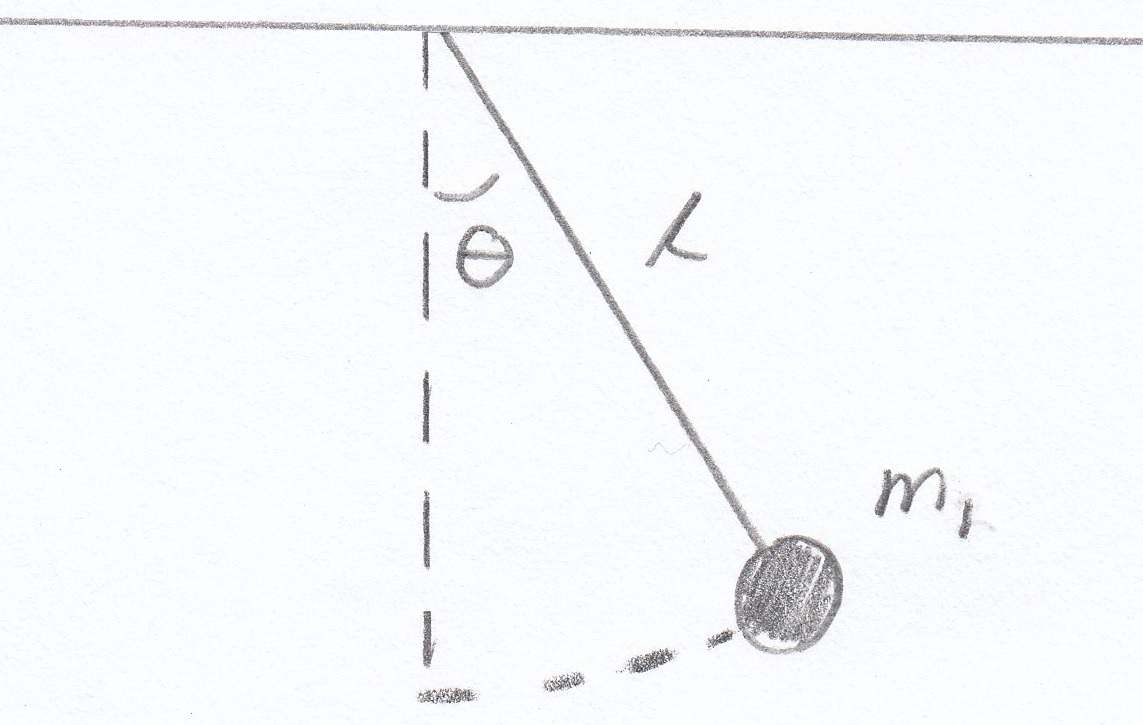
\includegraphics[width=0.3\textwidth]{figures/pen}
		\caption{The simple pendulum.}
		\label{fig:pen}
	\end{figure}
	From Newtons second law
	\begin{equation}
		\vec{F}_{res}=m_1\vec{a}
		=\vec{F}_g+\vec{F}_s,
	\end{equation} 
	where $\vec{F}_s$ is the force from the string onto the mass, $m_1$. $m_1$ does not move in the radial direction, so $\vec{F}_s$ must cancel the part of $\vec{F}_g$ in the radial direction,  i.e.
	\begin{equation}
		|\vec{F}_s|=-|\vec{F}_g|cos(\theta).
	\end{equation} 
	Therefore
	\begin{equation}
		m_1|\vec{a}|=-|\vec{F}_g|sin(\theta).
	\end{equation} 
	Now, $\vec{a}$ is the linear acceleration, in terms of the angular acceleration; $|\vec{a}|=\ddot{\theta}l$. Taking the small angle limit ($sin(\theta)\simeq \theta$), and using that $|\vec{F}_g|=m_1g$
	\begin{equation}
		\ddot{\theta}+\frac{g}{l}\theta\simeq 0\Rightarrow \theta\simeq \theta_0cos\bigg(\sqrt{\frac{g}{l}t}\bigg).
	\end{equation} 
	
\end{example}

\section{Non-inertial reference frames}
\index{Non-inertial reference frames}
When considering non-inertial reference frames it is desired to relate the force in a non-inertial reference frame to the forces in an inertial reference frame. Hence, the procedure of interest is how to transform Newtons second law from an inertial reference frame to a non-inertial reference frame. For this reason, a particle is considered from two different coordinate systems. One coordinate system, I, is an inertial reference frame that describes the location of the particle in terms of the position vector, $\vec{x}$. The non-inertial reference frame, I', performs a translating and rotating motion with respect to I. The distance from Origo in I to Origo in I' is defined by the vector $\vec{x}_0$, while the distance from Origo in I' to the particle is denoted by the vector $\vec{x'}$ (see figure \ref{fig:ref}).
\begin{figure}[h]
	\captionsetup{width=1\textwidth}
	\centering
	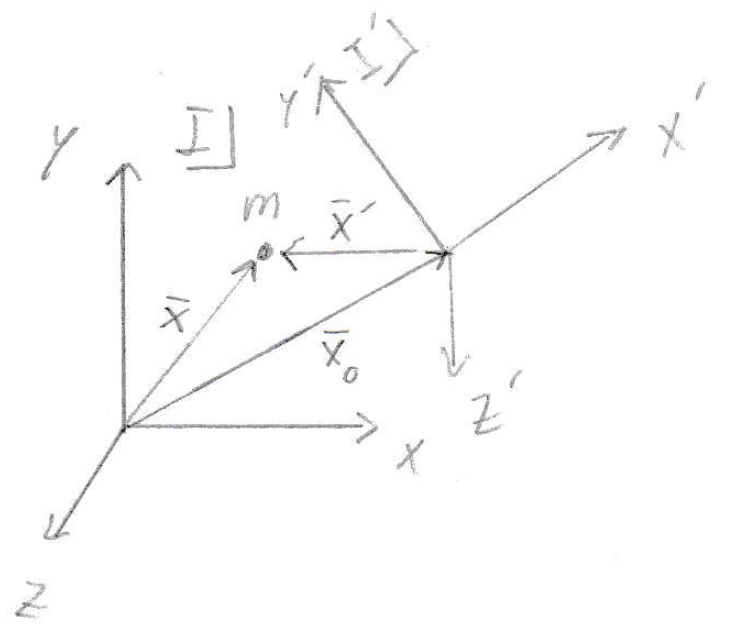
\includegraphics[width=0.5\textwidth]{figures/ref}
	\caption{The definition of the inertial an non-inertial reference frames, I,I', respectively.}
	\label{fig:ref}
\end{figure}
The two coordinate system could for example be the heliocentric reference frame as the inertial reference frame and the geocentric reference frame as the non-inertial reference frame\footnote{Depending on which approximations are made. Often the geocentric reference frame is taken to be an inertial reference frame. This is a valid approximation as long as the physical experiment under consideration does not span a significant portion of the Earth, i.e. as long as the experiment is confined to a smaller region of the Earth.}. From the definitions made in figure \ref{fig:ref} the position vector, $\vec{x}$, can be expressed in terms of $\vec{x}_0$ and $\vec{x'}$ viz
\begin{equation}
	\vec{x}=\vec{x}_0+\vec{x'}.
	\label{x1}
\end{equation} 
Equation \eqref{x1} can be used to relate the acceleration on $m_1$ as seen from I, I' by differentiating it twice with respect to time
\begin{equation}
	\begin{split}
		\ddot{\vec{x}}=\ddot{\vec{x}}_0+\ddot{\vec{x'}}+\vec{\omega}\times (\vec{\omega}\times \vec{x'})+2(\vec{\omega}\times \dot{\vec{x'}})+\dot{\vec{\omega}}\times \vec{x'}.
	\end{split}
	\label{x2}
\end{equation} 
By multiplying with the mass of the particle, and isolating $\vec{F}_{res,I'}=m\ddot{\vec{x'}}$ from equation \eqref{x2}
\begin{equation}
	\begin{split}
		\vec{F}_{res,I'}&=m\ddot{\vec{x'}}\\
		&=m[\ddot{\vec{x}}-\ddot{\vec{x}}_0-\vec{\omega}\times (\vec{\omega}\times \vec{x'})-2(\vec{\omega}\times \dot{\vec{x'}})-\dot{\vec{\omega}}\times \vec{x'}],\\
	\end{split}
	\label{x3}
\end{equation} 
where $\omega$ is the angular velocity of a given rotation around the axis going through the origin in I'. From equation \eqref{x3} it is clear that the resulting force in the reference frame of I' is equal to the resulting force in I subtracted some terms. These subtracted terms are what is called fictitious forces. Fictitious" because the forces are not real in the sense that they appear in an inertial reference frame. The fictitious forces represent the movement of the non-inertial reference frame, and as such they do not originate from any other body (as inertial forces do). The fictitious forces are defined as follows
\begin{equation}
	\begin{split}
		&\text{Origins; linear acceleration of I', wrt. I:}\qquad \ddot{\vec{x}}_0,\\
		&\text{Centrifugal acceleration:}\quad\qquad\quad\qquad\qquad\,\,\,\, \vec{\omega}\times (\vec{\omega}\times \vec{x'}),\\
		&\text{Coriolis acceleration: }\qquad\quad\quad\qquad\quad\qquad\,\,\,\, 2(\vec{\omega}\times \dot{\vec{x'}}),\\
		&\text{Azimuthal acceleration: }\qquad\quad\quad\qquad\qquad\,\,\,\, \dot{\vec{\omega}}\times \vec{x'}.\\
	\end{split}
\end{equation} 
The linear acceleration term is the one experience when sitting inside an accelerating car. The centrifugal term is one which is experience on a marry-go-round. The Coriolis term is more obscure. It is a force experience by particles which move in a rotating reference frame. For example, one would experience the Coriolis force if one walked around on a rotating marry-go-round. If one walked towards the center of a marry-go-round one would experience the Coriolis force pushing from the side. The azimuthal term, also called the Euler term, is also an obscure term. It is experience if the angular velocity of the rotating reference frame is changed. For example it would be experienced if the marry-go-round's rotational velocity accelerated or decelerated. If walking towards the center of a marry-go-round that is accelerating in rotational velocity, the azimuthal force would act to the opposite side as that of the Coriolis force. From the above definitions, the resulting force in a non-inertial reference frame can be written viz
\begin{equation}
	\vec{F}_{res,I'}=\vec{F}_{res,I}+\vec{F}_{trans}+\vec{F}_{centr}+\vec{F}_{cor}+\vec{F}_{azi},
\end{equation} 
where the fictitious forces are defined to absorb the minus signs.

\section{Center of mass}
Consider a system of point particles observed from some inertial reference frame, I. The particles might be mutually interacting (eg. via the gravitational interaction or the electromagnetic interaction) such that they form a rigid body. A rigid body is defined as a body consisting of many particles which do not change position during movement of the rigid body. The center of mass, with respect to origin in the inertial coordinate system, of both a system of particles and a rigid body is found by summing the positions of the individual particles weighted with their individual masses and divided by the total mass,  i.e.
\begin{equation}
	\vec{x}_{CM}=\frac{1}{m_{tot}}\sum_{i}m_i\vec{x}_i,
	\label{y1}
\end{equation} 
where $m_{tot}=\sum_i m_i$. Differentiating equation \eqref{y1} with respect to time, and taking $m_{tot}$ to the left hand side, reveals
\begin{equation}
	\begin{split}
		m_{tot}\vec{v}_{CM}=\sum_im_i\vec{v}_i=\sum_i\vec{p}_i=\vec{p}.
	\end{split}
	\label{y2}
\end{equation} 
Equation \eqref{y2} informs that the total, linear momentum of a system of particles, i.e. $\vec{p}$, is the sum of the linear momenta of all the constituent particles. Differentiating equation \eqref{y2} once more with respect to time
\begin{equation}
	\begin{split}
		\vec{F}_{res}&=\frac{d \vec{p}}{dt}=\sum_i \frac{d \vec{p}_i}{dt}=\sum_i m_i\ddot{\vec{x}}_i.\\
	\end{split}
	\label{y3}
\end{equation} 
The resulting force can be divided into two categories; the external forces and the internal forces. The external forces is forces that originate from bodies outside the system of particles whereas internal forces are forces that originate between constituents of the system of particles. According to Newtons third law (the law of action and reaction); the force from any particle onto another results in an equal force with opposite direction the other way around. Hence, denoting the force between particles $i,j$ as $\vec{F}_{ij}$
\begin{equation}
	\vec{F}_{ij}=-\vec{F}_{ji}.
	\label{y4}
\end{equation} 
Using equation \eqref{y4} in equation \eqref{y3} it is clear that the contribution to the resulting force from the internal forces vanish, and so
\begin{equation}
	\vec{F}_{res}=\sum_i\vec{F}_{ext,i}.
	\label{y5}
\end{equation} 
\paragraph{Center of mass theorem:}\index{Center of mass theorem} \emph{Hence, the entire mass of a system of particles, rigid or not, behaves as if the entire mass were concentrated in the center of mass and all external forces act in this point (from equation \eqref{y5}).} 
\paragraph{Conservation of linear momentum:} \index{Conservation of linear momentum} \emph{If no external forces act on a system of particles the total momentum, $\vec{p}$, of the system is a constant vector (from equation \eqref{y5}, \eqref{y3}).} \newline


\section{Energy}
Consider a particle, observed from an inertial reference frame, moving under the influence of a generic force, $\vec{F}$, which is taken to be a function of any relevant variables. When the particle is moved, by the force, from point a to point b, the force performs an amount of work, $W_{AB}$, on the particle, given by
\begin{equation}
	W_{ab}=\int_{a}^{b}\vec{F}\cdot d\vec{x}=\int\vec{F}\cdot\hat{n} d^3x,
	\label{w1}
\end{equation} 
where $\hat{n}$ is the unit tangent vector along the path of integration, i.e. the path along which which the particle is moving. Using Newtons second law equation \eqref{w1} can be written as follows
\begin{equation}
	W_{ab}=\int_a^bm\frac{d\vec{v}}{dt}\cdot d\vec{x}=\int_{a}^{b}m\vec{v}\cdot d\vec{v}=\frac{1}{2}mv_b^2-\frac{1}{2}mv_a^2.
	\label{w2}
\end{equation} 
The quantity $T=\frac{1}{2}mv^2$ is defined as the kinetic energy of the particle. From equation \eqref{w2} it is clear that the work done by all force acting on a particle equals the increase in kinetic energy of the particle,  i.e.
\begin{equation}
	W=\int\vec{F}\cdot d\vec{x}=\Delta T\Rightarrow dT=\vec{F}\cdot d\vec{x}\Rightarrow \frac{dT}{dt}=\vec{F}\cdot \vec{v}.
	\label{w3}
\end{equation} 
$\vec{F}\cdot \vec{v}$ is defined as the power done by the force $\vec{F}$. Related to the work integral is the definition of a conservative force and a conservative force field. 
\paragraph{Conservative force fields:}\index{Conservative force fields} \emph{A force field is called conservative if the work integral, $W_{ab}=\int_{a}^{b}\vec{F}\cdot d\vec{x}$, is independent on the path of integration, and depends only on the initial and final points.}

\paragraph{Central force fields:} \index{Central force fields} \emph{A central force field is a field where the force on the particle is always directed towards (or away from) a point, fixed in an inertial reference frame. This point is called the force center. All central force fields are conservative force fields and as such central force fields are a subgroup of conservative force fields.}\newline

A particle in a conservative force field has associated to it a potential energy, $V=V(\vec{x})$. The potential energy is defined with respect to some reference point and the notion of the "total potential energy" is senseless. Taking $U(P)=0$, the potential energy of a particle at point $a$ (in a conservative force field), is given by 
\begin{equation}
	V(\vec{a})=-\int_{P}^{a}\vec{F}\cdot d\vec{x}=-W_{ab}\Rightarrow \vec{F}=-\vec{\nabla}V(\vec{x}),
	\label{w4}
\end{equation}  
where $\vec{\nabla}=\begin{bmatrix}
	\partial_x & \partial_y & \partial _z\\
\end{bmatrix}^T$ is the gradient operator\footnote{A mathematical operator. Not to be confused with a quantum mechanical operator}. From equation \eqref{w4} it is clear that the potential energy is equal to minus the work done in moving a particle between two points. So, one can think of the potential energy as a means to store work. Consider now two arbitrary points in a conservative force field ($a,b$). For these points
\begin{equation}
	\int_P^a\vec{F}\cdot d\vec{x}=-V(a), \quad \int_P^b\vec{F}\cdot d\vec{x}=-V(b).
	\label{w5}
\end{equation} 
From equation \eqref{w5}
\begin{equation}
	\int_{a}^{b}\vec{F}\cdot d\vec{x}=\int_a^P\vec{F}\cdot d\vec{x}+\int_P^b\vec{F}\cdot d\vec{x}=V(a)-V(b).
	\label{w6}
\end{equation} 
Comparing equation \eqref{w6} to equation \eqref{w2}
\begin{equation}
	\frac{1}{2}mv_b^2-\frac{1}{2}mv_a^2=V(a)-V(b)\Rightarrow \frac{1}{2}mv_b^2+V(b)=\frac{1}{2}mv_a^2+V(a).
	\label{w8}
\end{equation}  
From equation \eqref{w8} it is clear that the sum of the kinetic and potential energy does not change as as the particle is moved, by a force, through a conservative force field. The sum of the kinetic and potential energy is defined as the mechanical energy, $E_{mek}$, so
\begin{equation}
	\text{In a conservative force field:}\quad E_{mek}=T+V=const.
\end{equation} 
\begin{example}
	\emph{A professional skier is skiing downhill  along the slope shown in figure \ref{fig:ski}. 
		\begin{figure}[H]
			\captionsetup{width=1\textwidth}
			\centering
			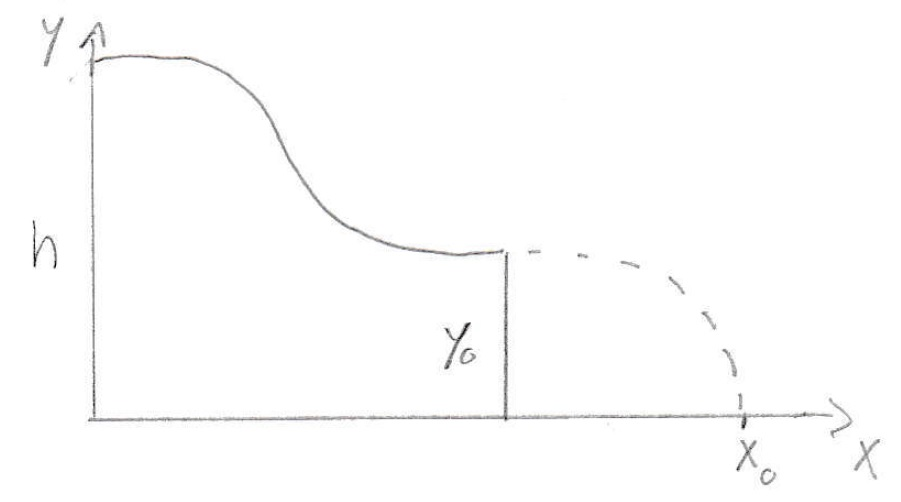
\includegraphics[width=0.3\textwidth]{figures/ski}
			\caption{The scenario of the ski-jumper.}
			\label{fig:ski}
		\end{figure}	
		The skier begins at $h=10m$ with $v=0\frac{m}{s}$. Assuming that there is no friction between the skies and the snow the skier arrives at the horizontal trampoline  with height $y_0$. Jumping out the skier lands at a distance $x_0$ from the horizontal trampoline.}
	
	\begin{enumerate}
		\item \emph{Determine the value of the trampoline hight, $y_0$, which maximizes $x_0$.}
		
		Since the skier is at rest when initiating the descend, from conservation of mechanical energy (no friction forces)
		\begin{equation}
			E_{mek}=mgh=\frac{1}{2}mv_0^2+mgy_0\Rightarrow v_0=\sqrt{2g(h-y_0)}.
		\end{equation} 
		Next use that the skier exits the jump at a horizontal direction. Subsequent to exiting the jump, the only force the skier is subject to is gravity. Since the gravitational acceleration is constant close to the Earth, the skier will take a time, $t_0$, before landing, given by
		\begin{equation}
			y_0=\frac{1}{2}gt_0^2\Rightarrow t_0=\sqrt{\frac{2y_0}{g}}.
		\end{equation} 
		During this time, the horizontal distance traversed is given by
		\begin{equation}
			x_0=v_0t_0\Rightarrow x_0=\sqrt{2g(h-y_0)}\sqrt{\frac{2y_0}{g}}=2\sqrt{hy_0-y_0^2}.
		\end{equation} 
		To maximize $x_0(y_0)$, isolate $y_0$ from $\frac{d x_0(y_0)}{dy_0}=0$ as follows
		\begin{equation}
			\frac{d x_0(y_0)}{dy_0}=\frac{h-2y_0}{\sqrt{hy_0-y_0^2}}=0 \Rightarrow y_0=\frac{h}{2}=5m.
		\end{equation} 
		$\frac{d^2x_0(y_0)}{dy_0^2}<0$ is indeed the case, so the point is a local maximum - Just as intended. This means $y_0=\frac{h}{2}=5m$ maximizes $x_0$.
		
		\item \emph{Determine the velocity of the skier when leaving the trampoline ($v_0$), and the distance in free air ($x_0$).}
		
		\begin{equation}
			\begin{split}
				&v_0=\sqrt{2g(h-\frac{h}{2})}=9.9\frac{m}{s},\\
				&x_0=\sqrt{2h^2-h^2}=10m.
			\end{split}
		\end{equation} 
	\end{enumerate}
\end{example}
\begin{example}
	\emph{An experienced mountaineer, which weights $m=80kg$, is climbing a near vertical wall. The mountaineer is secured against a possible fall by a climbing robe. One end of the robe is attached to the mountaineer while the other is secured by a pole in the rock below the mountaineer. The mountaineer climbs sufficiently high that he has used up the full length of the rope, $l_0$, which is still not stretched. This fill length of the rope is therefore identical to the difference in height between the mountaineer and the second pole below him. Assume negligible rope weight, and that the rope behaves as an ideal string with elastic constant $K=\frac{a}{l_0}$, with $a=40000N$.}
	
	\begin{enumerate}
		\item \emph{Determine the maximum tension of the rope if the mountaineer falls.}
		
		The physical scenario is modeled as shown in figure \ref{fig:moun}.
		\begin{figure}[H]
			\captionsetup{width=1\textwidth}
			\centering
			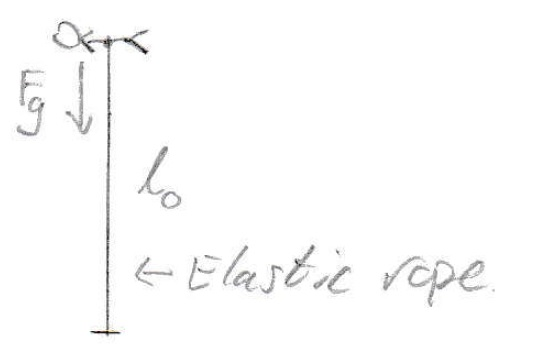
\includegraphics[width=0.3\textwidth]{figures/moun}
			\caption{The scenario of the mountaineer.}
			\label{fig:moun}
		\end{figure}
		Use that the maximum force from the rope is given by
		\begin{equation}
			F_{max}=kx_{max},
		\end{equation} 
		where $x_{max}$ is found by using the conservation of energy. The mountaineer initiates the fall with only potential energy. Subsequent to falling the mountaineer will stretch the rope and at some point, at which time the rope will eb stretched maximally, come to rest. When the rope is stretched maximally the tension of the rope will be at its highest, so 
		\begin{equation}
			\begin{split}
				E_{pot}&=mg(2l_0+x_{max})=\frac{1}{2}kx_{max}^2\\
				&\Rightarrow x_{max}=\frac{mg+\sqrt{(mg)^2+4Kmgl_0}}{k}\\
				&\Rightarrow F_{max}=mg+\sqrt{(mg)^2+4kmgl_0}\simeq 12 015 N.
			\end{split}
		\end{equation} 
	\end{enumerate}
\end{example}

\section{Angular momentum in classical mechanics}
Consider a particle of mass $m$ moving with a velocity $\vec{v}$ relative to some inertial reference frame I with origins in the point O. Relative to the point O, the angular momentum is defined as
\begin{equation}
	\vec{L}=\vec{x}\times \vec{p}=m\vec{x}\times \vec{v}=m rvsin(\theta),
	\label{ll1}
\end{equation} 
where $r=|\vec{x}|$ and $\theta$ is the angle between $\vec{v}$ and $\vec{x}$. The cross product multiplies the radius vector with the part of the velocity that is perpendicular to the radius vector. Differentiating equation \eqref{ll1} with respect to time reveals
\begin{equation}
	\frac{d\vec{L}}{dt}=\frac{d}{dt}(\vec{x}\times \vec{p})=\frac{d\vec{x}}{dt}\times \vec{p}+\vec{x}\times \frac{d\vec{p}}{dt}.
	\label{ll2}
\end{equation} 
Since $\frac{d\vec{x}}{dt}=\vec{v}\parallel \vec{p}$ the first term in equation \eqref{ll2} vanishes and so
\begin{equation}
	\frac{d\vec{L}}{dt}\vec{x}\times \frac{d\vec{p}}{dt}=\vec{x}\times\vec{F}.
\end{equation} 
The product $\vec{x}\times\vec{F}$ is defined as torque, $\vec{N}$, so
\begin{equation}
	\vec{N}\equiv \vec{x}\times\vec{F}=\frac{d\vec{L}}{dt}.
	\label{ll3}
\end{equation}  
\paragraph{The angular momentum theorem:}\index{Angular momentum theorem} \emph{The rate of change of the angular momentum of a particle around some point, O, equals the torque on the particle, with respect to O.}

\paragraph{Conservation of angular momentum:}\index{Conservation of angular momentum} \emph{If no torque acts on a particle, the angular momentum, around some point O, of that particle, with respect to the point O, is constant in time.}

\begin{example}
	A classic example of a system in which angular momentum is conserved is a central force field, eg. the gravitational field of a point particle. 
\end{example}
\begin{example}
	The angular momentum of a closed system, i.e. a system upon which no external forces act, is conserved. 
\end{example}

For a system of particles torque is given by
\begin{equation}
	\vec{N}_{res}=\sum_i\vec{N}_i=\sum_i\frac{d\vec{L}_i}{dt},
\end{equation} 
where $i$ runs over both external and internal forces. From Newtons third law $\vec{F}_{ij}=-\vec{F}_{ji}$, so for the internal torque
\begin{equation}
	\vec{N}_{ij}=\vec{x}_i\times \vec{F}_{ij}+\vec{x}_j\times \vec{F}_{ji}=(\vec{x}_i-\vec{x}_j)\times \vec{F}_{ij}=\vec{0}.
\end{equation} 
Hence, analogous to the case of Newtons second law for linear motion in which the resulting force was indifferent to the internal forces; the resulting torque is indifferent to the internal torques, so
\begin{equation}
	\vec{N}_{res}=\sum_{i}\vec{N}_{ext,i}.
\end{equation} 

\begin{example}
	\index{Planetary physics in Newtonian limit}
	\emph{Halley's comet is the most famous of all comets. It has a period of $76$ years and has been observed regularly since the battle of Hastings in $1066$. It has, in the point where it is closest to the Sun, a distance $r_0$ to the Sun, and a velocity $v_0$ relative to the heliocentric reference frame.}
	
	\begin{enumerate}
		\item \emph{Find a formal expression of the areal velocity of the comet, $\frac{dA}{dt}$, expressed in terms of $r_0$ and $v_0$.}
		
		Use that the cross product between two vectors denotes the area of the parallelogram they enclose (see figure \ref{fig:par}).
		\begin{figure}[h]
			\captionsetup{width=1\textwidth}
			\centering
			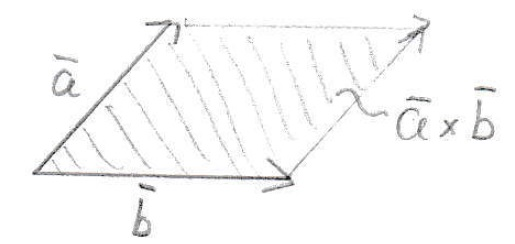
\includegraphics[width=0.3\textwidth]{figures/par}
			\caption{The parallelogram of the cross product.}
			\label{fig:par}
		\end{figure}
		The vectors relevant for the parallelogram in the physical scenario is $\vec{v}(t)$ and $\vec{r}(t+\Delta t)$ (see figure \ref{fig:par2}).
		\begin{figure}[h]
			\captionsetup{width=1\textwidth}
			\centering
			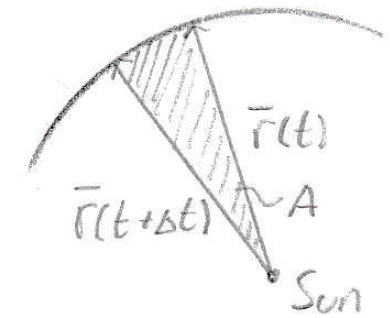
\includegraphics[width=0.3\textwidth]{figures/par2}
			\caption{The area under consideration.}
			\label{fig:par2}
		\end{figure}
		From figure \ref{fig:par2}
		\begin{equation}
			\Delta A=\frac{\vec{r}(t)\times \vec{r}(t+\Delta t)}{2}
			\label{A1}
		\end{equation} 
		Dividing equation \eqref{A1} by $\Delta t$ and taking the limit of $\Delta t\Rightarrow 0$
		\begin{equation}
			\begin{split}
				\frac{dA}{dt}&=\lim\limits_{\Delta t\Rightarrow 0}\bigg(\frac{\Delta A}{\Delta t}\bigg)=\lim\limits_{\Delta t\Rightarrow 0}\bigg(\frac{\vec{r}(t)\times \vec{r}(t+\Delta t)}{2\Delta t}\bigg)\\
				&=\lim\limits_{\Delta t\Rightarrow 0}\bigg(\frac{\vec{r}(t)\times (\vec{r'}(t)+\dot{\vec{r}}(t)\Delta t)}{2\Delta t}\bigg)\\
				&=\lim\limits_{\Delta t\Rightarrow 0}\bigg(\frac{\vec{r}(t)\times \dot{\vec{r}}(t)}{2}\frac{\Delta t}{\Delta t}\bigg)=\frac{\vec{r}(t)\times \vec{v}(t)}{2},\\
			\end{split}
		\end{equation} 
		where it has been used that $\vec{r}(t)\times \vec{r}(t)=\vec{0}$. Since the area velocity is constant the values of $v,r$ at the closest approach to the Sun can be used. At closest approach $\vec{v}_0\perp\vec{r}_0$, so
		\begin{equation}
			\frac{dA}{dt}=\frac{r_0v_0}{2}.
		\end{equation} 
		Alternatively, angular momentum can be used to obtain the same result. Consider figure \ref{fig:an}
		\begin{figure}[h]
			\captionsetup{width=1\textwidth}
			\centering
			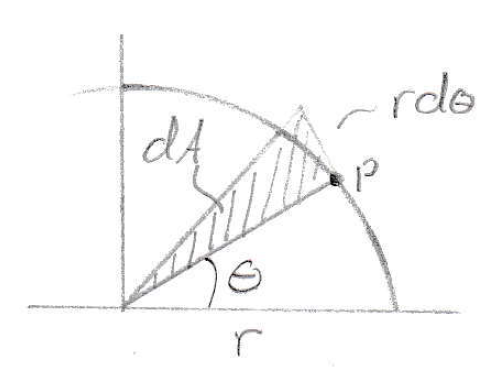
\includegraphics[width=0.3\textwidth]{figures/an}
			\caption{The orbit in polar coordinates.}
			\label{fig:an}
		\end{figure}
		From figure \ref{fig:an}
		\begin{equation}
			dA=\frac{1}{2}r^2d\theta\Rightarrow \frac{dA}{dt}=\frac{1}{2}r^2\frac{d\theta}{dt}.
			\label{r4}
		\end{equation} 
		To determine $\frac{d\theta}{dt}$ use conservation of angular momentum. The equation of motion for the comet is given by
		\begin{equation}
			m_C\ddot{\vec{r}}=-\frac{G_Nm_Cm_\odot}{|\vec{r}|^2}\frac{\vec{r}}{|\vec{r}|},
			\label{r1}
		\end{equation} 
		where $m_C$ is the mass of the comet and $m_\odot$ is the mass of the Sun. In polar coordinates
		\begin{equation}
			\ddot{\vec{r}}=\bigg(|\ddot{\vec{r}}|-|\vec{r}|\bigg(\frac{d\theta}{dt}\bigg)^2\bigg)\hat{e}_r+\frac{1}{|\vec{r}|}\frac{d}{dt}\bigg(|\vec{r}|^2\frac{d\theta}{dt}\bigg)\hat{e}_\theta.
			\label{r2}
		\end{equation} 
		Using equation \eqref{r2} in equation \eqref{r1} results in two equations; a radial and an angular
		\begin{equation}
			\begin{split}
				&\text{Radial:} \quad m_C\bigg(|\ddot{\vec{r}}|-|\vec{r}|\bigg(\frac{d\theta}{dt}\bigg)^2\bigg)\hat{e}_r=-\frac{G_Nm_Cm_\odot}{|\vec{r}|^2}\hat{e}_r,\\
				&\text{Angular:} \quad \frac{1}{|\vec{r}|}\frac{d}{dt}\bigg(|\vec{r}|^2\frac{d\theta}{dt}\bigg)\hat{e}_\theta=0.\\
			\end{split}
			\label{shi}
		\end{equation} 
		From the angular equation
		\begin{equation}
			\begin{split}
				\frac{d}{dt}\bigg(|\vec{r}|^2m_C\dot{\theta}\bigg)=0&\Rightarrow m_C|\vec{r}|^2\dot{\theta}=const\equiv L\\
				&\Rightarrow \dot{\theta}=\frac{L}{m_Cr^2},\\
			\end{split}
			\label{r3}
		\end{equation} 
		where $r=|\vec{r}|$. Using equation \eqref{r3} in equation \eqref{r4}
		\begin{equation}
			\frac{dA}{dt}=\frac{L}{2m_C}=\frac{m_C\vec{r}\times \vec{v}}{2m_C}=\frac{r_0v_0}{2}.
			\label{r15}
		\end{equation} 
		
		\item \emph{Find formal expressions of the angular momentum, $L$, and the total energy, $E_{mek}$, of the comet. From these two expressions obtain expressions for the eccentricity, $e$, the semi-major axis of the comets orbit, $a$, and the period, $T$, of the orbital motion. All expressions should be formulated in terms of $r_0$, $v_0$, $m_\odot$ and $G_N$.}
		
		Begin by considering the radial equation (equation \eqref{shi}). Substituting equation \eqref{r3} into the radial equation of equation \eqref{shi}
		\begin{equation}
			m_C\ddot{r}-r\frac{L^2}{m_Cr^4}=-\frac{G_Nm_Cm_\odot}{r^2}\Rightarrow \ddot{r}-\frac{L^2}{m_C^2r^3}=\frac{C}{m_Cr^2},
			\label{r5}
		\end{equation} 
		where $C\equiv-G_Nm_Cm_\odot$. Equation \eqref{r5} is a differential equation for $r(t)$, however, in relation to the orbit the quantity of interest is not $r(t)$, but rather $r(\theta)$. To introduce $r(\theta)$ into equation \eqref{r5}, use that
		\begin{equation}
			\begin{split}
				\ddot{r}&=\frac{d}{dt}\bigg(\frac{dr}{dt}\bigg)=\frac{d}{dt}\bigg(\frac{dr}{d\theta}\frac{d\theta}{dt}\bigg)=\frac{d}{dt}\bigg(\frac{dr}{d\theta}\frac{L}{m_Cr^2}\bigg)\\
				&=\frac{d}{d\theta}\bigg(\frac{dr}{d\theta}\frac{L}{m_Cr^2}\bigg)\frac{d\theta}{dt}=\frac{L^2}{m_C^2r^4}\frac{d^2r}{d\theta^2}+\frac{L^2}{m_C^2r^2}\bigg(-2r^{-3}\frac{dr}{d\theta}\bigg)\frac{dr}{d\theta}\\
				&=\frac{L^2}{m_C^2r^4}\bigg(\frac{d^2r}{d\theta^2}-\frac{2}{r}\bigg(\frac{dr}{d\theta}\bigg)^2\bigg).
			\end{split}
			\label{r6}
		\end{equation} 
		Next, introduce the variable $u=r^{-1}$, for which
		\begin{equation}
			\begin{split}
				\frac{d^2u}{d\theta^2}&=\frac{d}{d\theta}\bigg(\frac{du}{d\theta}\bigg)=\frac{d}{d\theta}\bigg(\frac{du}{dr}\frac{dr}{d\theta}\bigg)=\frac{d}{d\theta}\bigg(-r^{-2}\frac{dr}{d\theta}\bigg)\\
				&=\frac{d}{dr}\bigg(-r^{-2}\bigg)\bigg(\frac{dr}{d\theta}\bigg)^2+(-r^{-2})\frac{d^2r}{d\theta^2}\\
				&=\frac{2}{r^3}\bigg(\frac{dr}{d\theta}\bigg)^2-\frac{1}{r^2}\frac{d^2r}{d\theta^2}\\
				&=-\frac{1}{r^2}\bigg(\frac{d^2r}{d\theta^2}-\frac{2}{r}\bigg(\frac{dr}{d\theta}\bigg)^2\bigg).
			\end{split}
			\label{r7}
		\end{equation} 
		Comparing equation \eqref{r6} and \eqref{r7}
		\begin{equation}
			\ddot{r}=-\frac{L^2}{m_C^2r^2}\frac{d^2u}{d\theta^2}.
			\label{r8}
		\end{equation} 
		Using equation \eqref{r8} in equation \eqref{r5}, alongside the definition of $u=r^{-1}$
		\begin{equation}
			-\frac{L^2}{m_C^2}u^2\frac{d^2u}{d\theta^2}-\frac{L^2}{m_C^2}u^3=\frac{C}{m_C}u^2\Rightarrow \frac{d^u2}{d\theta^2}+u=-\frac{Cm_C}{L^2}.
			\label{r9}
		\end{equation} 
		Equation \eqref{r9} is an inhomogeneous, second order, linear, ordinary differential equation. The solution is a sum of \emph{one} solution to the inhomogeneous equation ($u_p$) and \emph{the} solution to the homogeneous equation ($u_h$). \emph{One} solution to the inhomogeneous equation is
		\begin{equation}
			u_p=-\frac{Cm_C}{L^2}.
		\end{equation} 
		The solution to the homogeneous equation is found via the conventional means (see \citealt{calculus})
		\begin{equation}
			u_h=Acos(\theta+\phi_0),
		\end{equation} 
		where $\phi_0$ is some phase. Hereby	
		\begin{equation}
			u=Bcos(\theta+\phi_0)-\frac{Cm_C}{L^2}.
			\label{r10}
		\end{equation} 
		By an appropriate placement of the coordinate system, $\phi_0=0$. To determine the integration-constant, $B$, initial conditions must be applied, or alternatively conservation laws. From conservation of energy
		\begin{equation}
			E_{mek}=\frac{1}{2}m_Cv^2+\frac{C}{r}=\frac{1}{2}m(\dot{r}^2+r^2\dot{\theta})+\frac{C}{r},
		\end{equation} 
		where polar coordinates have been used to express $v$. Using $\dot{\theta=\frac{L}{m_Cr^2}}$, from equation \eqref{r3}, the mechanical energy can be written as follows
		\begin{equation}
			E_{mek}=\frac{L^2}{2m_Cr^4}\bigg(\bigg(\frac{dr}{d\theta}\bigg)^2+r^2\bigg)+\frac{C}{r}.
			\label{r11}
		\end{equation} 
		Using equation \eqref{r10} in equation \eqref{r11}
		\begin{equation}
			\begin{split}
				\frac{dr}{d\theta}&=\frac{1}{B}\frac{sin(\theta)}{cos(\theta)^2}=Br^2sin(\theta)\\
				&\Rightarrow E_{mek}=\frac{L^2}{2m_Cr^4}\bigg(B^2r^4sin(\theta)^2+r^2\bigg)+\frac{C}{r}.\\
			\end{split}
			\label{r12}
		\end{equation} 		
		Using again equation \eqref{r10} in equation \eqref{r12}
		\begin{equation}
			E_{mek}=\frac{L^2B^2}{2m_C}-\frac{C^2m_C}{2L^2}\Rightarrow B=\sqrt{\bigg(E_{mek}+\frac{C^2m_C}{2L^2}\bigg)\frac{2m_C}{L^2}}.
			\label{r13}
		\end{equation} 
		Using equation \eqref{r13} in equation \eqref{r10}
		\begin{equation}
			\frac{1}{r}=\sqrt{\frac{2m_CE_{mek}}{L^2}+\frac{G_N^2m_\odot^2m_C^4}{L^4}}cos(\theta)+\frac{G_Nm_C^2m_\odot}{L^2}.
			\label{r14}
		\end{equation} 
		Equation \eqref{r14} can be written on the form of an ellipse equation,  i.e.
		\begin{equation}
			\frac{1}{r}=\frac{1}{p}(1+e\cdot cos(\theta)),
		\end{equation} 
		where
		\begin{equation}
			\begin{split}
				&p=\frac{L^2}{G_Nm_C^2m_\odot},\\
				&e=\sqrt{1+\frac{2E_{mek}L^2}{G_N^2m_C^3m_\odot^2}},
			\end{split}
		\end{equation} 
		where $e$ is the eccentricity of the orbit and $p$ is half the length of the chord perpendicular to the axis of the conic section and passing through the focus point. To get some results, use that from equation \eqref{r15}
		\begin{equation}
			\frac{dA}{dt}=\frac{L}{2m_c}\Rightarrow A=\frac{LT}{2m_C}=\pi ab=\pi a^2\sqrt{1-e^2},
			\label{r16}
		\end{equation} 
		where $a$ is the length of the semi-major axis, $b$ is the length of the semi-minor axis, $A=\pi ab$ is the area of an ellipse and $b=a\sqrt{1-e^2}$ is valid for an ellipse. Next use that
		\begin{equation}
			\begin{split}
				p&=a(1-e^2)=\frac{L^2}{G_Nm_c^2m_\odot}\\
				&\Rightarrow a=\frac{L^2}{G_Nm_C^2m_\odot}\frac{1}{1-e^2}=\frac{G_Nm_Cm_\odot}{2|E_{mek}|}.
			\end{split}
			\label{r17}
		\end{equation} 
		Using equation \eqref{r17} in equation \eqref{r16}
		\begin{equation}
			\begin{split}
				A&=\frac{LT}{2m_C}=\pi\bigg(\frac{G_Nm_Cm_\odot}{2|E_{mek}|}\bigg)^2\sqrt{1-e^2}\\
				&=\pi\bigg(\frac{G_Nm_Cm_\odot}{2|E_{mek}|}\bigg)^2\sqrt{\frac{2|E_{mek}|L^2}{G_N^2m_C^3m_\odot^2}}\\
				&=\pi G_NM_\odot L\sqrt{m_c}(2|E_{mek}|)^{-\frac{3}{2}}=\frac{\pi G_N m_\odot v_0r_0}{\big(v_0^2-\frac{2G_Nm_\odot}{r_0}\big)^{\frac{3}{2}}},
			\end{split}
		\end{equation} 
		where $L,E_{mek}$ has been inserted for the last equality. Using $E_{mek}$ in equation \eqref{r17}
		\begin{equation}
			a=\frac{G_N M_\odot m_C}{2|E_{mek}|}=\frac{1}{\frac{v_0^2}{G_Nm_\odot}-\frac{2}{r_0}}
		\end{equation} 
		Lastly, the period of the orbit:
		\begin{equation}
			T=\frac{2m_CA}{L}=\frac{2\pi G_N m_\odot}{\big(v_0^2-\frac{2G_Nm_\odot}{r_0}\big)^{\frac{3}{2}}}
		\end{equation} 
		
		\item \emph{Find numerical values for $e$ and $T$ by using $r_0=0.5870 AU$, $1AU= 1.496\cdot 10^9m$, $v_0=54.53\frac{km}{s}$, $G_N=6.76\cdot 10^{-11}\frac{Nm^2}{kg^2}$ and $m_\odot=1.989\cdot 10^30kg$.}
		
		By inserting the numbers:
		\begin{equation}
			\begin{split}
				&a=\frac{G_Nm_\odot}{2|\frac{1}{2}v_0^2-\frac{G_Nm_\odot}{r_0}|}\simeq 2.69\cdot 10^9 km\simeq 18 AU\\
				&e=\sqrt{1+\frac{v_0^4r_0^2-2G_Nm_\odot v_0^2r_0}{G_N^2m_\odot^2}}\simeq 0.967\\
				&T=\frac{2\pi a^2\sqrt{1-e^2}}{r_0v_0}\simeq 76.28\, years
			\end{split}
		\end{equation} 		
	\end{enumerate}
\end{example}

\begin{example}
	\index{Planetary physics in Newtonian limit}
	\emph{The Enterprise's last tour into darkness has been completed. After the last deep-space mission the spaceship has re-entered the Solar system. It is now on a circular orbit of radius $R_0$ around the Earth. The Enterprise has velocity $\vec{v}_0$ with respect to the reference frame with origin in the center of the Earth and the axis towards what seems to be the fixed stars in the night sky. Consider this reference frame to be inertial. Upon the sudden news that a new super villain is attacking the headquarters of the intergalactic confederation fleet, the Enterprise moves from a circular orbit of radius $R_0$ to another, elliptical orbit, with perigee, $P$, at a distance, $R$, from the center of the Earth. During this maneuverer the Enterprise expels the mass $m_1$ of fuel while acquiring the velocity $\vec{v}_1=\vec{v}_0+\Delta\vec{v}$ with $\Delta\vec{v}$ in the direction of the Earths center. When the Enterprise passes through the perigee, $P$, again, it ejects fuel of mass $m_2$ to acquire the escape velocity tangent to the elliptic orbit. 
		In all the cases considered above, assume, for simplicity, that the fuel is expelled instantaneously and that the modulus of its speed relative to the Enterprise,	after been expelled, is $v_r$. Lieutenant Commander Spock (you) acquires the following data from the command deck: $R=0.91R_0$ and $v_r=2\sqrt{\frac{G_NM_E}{R_0}}$. 
		James T. Kirk, the commander of the Enterprise, asks the Lieutenant Commander Spock (you):}
	
	\begin{enumerate}
		\item \emph{What is the ratio between the mass $m_1+m_2$ of fuel consumed and the total mass, $m_s$, of the Enterprise?}
		
		The physical scenario is shown in figure \ref{fig:ent}.		
		\begin{figure}[h]
			\captionsetup{width=1\textwidth}
			\centering
			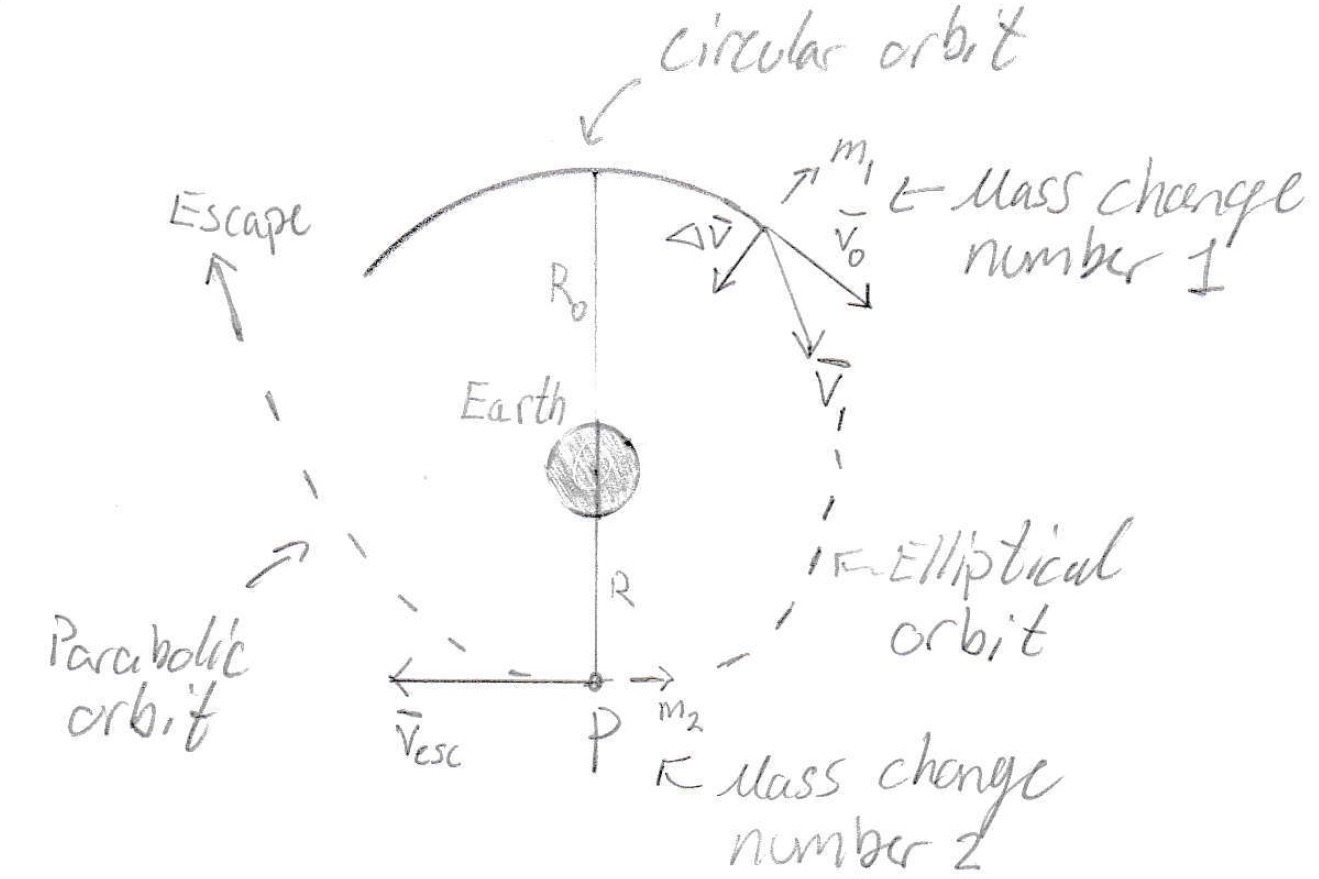
\includegraphics[width=0.8\textwidth]{figures/ent}
			\caption{The scenario of the Enterprise.}
			\label{fig:ent}
		\end{figure}
		The goal is to determine: $\text{Ratio 1}=\frac{m_1+m_2}{m_s}$. To do so, $m_1$ must be specified in terms of $m_2$ and $m_s$ must be specified in terms of $m_1,m_2$. The plan is to use conservation of linear and angular momentum to do so. Conservation across the first ejection of mass dictates:
		\begin{equation}
			\begin{split}
				m_s\vec{v}_0&=(m_s-m_1)(\vec{v}_0+\Delta\vec{v}_1)+m_1\vec{u}_1\\
				&=m_s\vec{v}_0+m_s\Delta\vec{v}_1+m_1(\vec{u}_1-\vec{v}_0-\Delta\vec{v}_1)\\
				&=m_s\vec{v}_0+m_s\Delta\vec{v}_1+m_1\vec{v}_r\\
				&\Rightarrow \Delta \vec{v}_1=-\frac{m_1}{m_s}\vec{v}_r\\
			\end{split}
		\end{equation} 
		where $\Delta \vec{v}_i$ denotes the velocity gained, $\vec{u}_i$ denotes the velocity of the fuel with respect to the (approximated) inertial reference frame of the Earth and $\vec{v}_r=\vec{u}-\vec{v}_0-\Delta\vec{v}_1$ is the relative velocity between the Enterprise and the fuel after it has been ejected. $\Delta \vec{v}_1\perp \vec{v}_0$, so $v_1^2=v_0^2+\Delta v_1^2+2\vec{v}_0\cdot \Delta \vec{v}_1=v_0^2+\Delta v_1^2=v_0^2+\big(\frac{m_1}{m_s}v_r\big)^2$. Hence, $v_1(v_0,m_1,m_s)$ has been determined. In order to determine the relation between $m_1$ and $m_s$, another (independent) equation for $v_1$ must be obtained. Such an equation comes from energy conservation between ejection of $m_1$ and $m_2$:
		\begin{equation}
			\begin{split}
				E_{mek}&= \frac{1}{2}(m_s-m_1)v_1^2-\frac{G_N(m_s-m_1)m_E}{R_0}\\
				&=\frac{1}{2}(m_s-m_1)v_p^2-\frac{G_N(m_s-m_1)m_E}{0.91R_0}\\
			\end{split}
			\label{l3}
		\end{equation} 
		To express the gravitational potential energy in terms of the circular, orbital velocity, $v_0$, use that for a circular orbit the eccentricity vanishes,  i.e.
		
		\begin{equation}
			\begin{split}
				e&=\sqrt{1+\frac{2E_{mek}L^2}{G_N^2m_s^3m_E^2}}=0\\
				&\Rightarrow \frac{2E_{mek}L^2}{G_N^2m_s^3m_E^2}=-1\\
				&\Rightarrow E_{mek}=\frac{G_N^2m_s^3m_E^2}{2L^2}=-\frac{G_N^2m_sm_E^2}{2(R_0v_0)^2}\\
			\end{split}
		\end{equation} 
		\normalsize
		where $L=v_0R_0$ for a circular orbit. From this the velocity of the circular orbit can be determined:
		\begin{equation}
			E_{mek}=\frac{1}{2}m_sv_0^2-\frac{G_Nm_sm_E}{R_0}=-\frac{G_N^2m_E^2m_s}{2R_0^2v_0^2}\Rightarrow v_0=\sqrt{\frac{G_Nm_E}{R_0}}
			\label{v_0}
		\end{equation} 
		Using equation \eqref{v_0} in equation \eqref{l3}
		\begin{equation}
			\begin{split}
				v_p^2&=v_1^2+2v_0^2\bigg(\frac{1}{0.91}-1\bigg)\\
				&=v_0^2+\frac{2m_1}{m_s}v_0^2+2v_0^2\bigg(\frac{1}{0.91}-1\bigg)\\
				&=v_0^2\bigg[\bigg(\frac{2m_1}{m_s}\bigg)^2+\frac{2}{0.91}-1\bigg].\\
			\end{split}
			\label{l5}
		\end{equation} 
		$v_p$ can be determined from conservation of angular momentum between ejection of $m_1$ and $m_2$. Just after $m_1$ is ejected
		\begin{equation}
			\vec{L}_1=(M-m_1)\vec{R}_0\times \vec{v}_1.
		\end{equation} 
		The cross product multiplies $R_0$ with the part of $\vec{v}_1$ perpendicular to $\vec{R}_0$, so
		\begin{equation}
			L_1=(M-m_1)R_0v_0.
			\label{l1}
		\end{equation} 
		Just before the Enterprise ejects the second mass, $m_2$, at perigee
		\begin{equation}
			L_2=(M-m_1)Rv_p=0.91R_0v_p.
			\label{l2}
		\end{equation} 
		Equating equation \eqref{l1} and \eqref{l2}
		\begin{equation}
			v_0=0.91v_p.
			\label{l4}
		\end{equation} 
		Using equation \eqref{l4} in equation \eqref{l5} reveals
		\begin{equation}
			m_s=\frac{2\cdot 0.91}{1-0.91}m_1\simeq 20.22 m_1.
			\label{l6}
		\end{equation} 
		With equation \eqref{l6} in the bag only a relation between $m_1$ and $m_2$ is needed to determine the desired ratio. such an expression is obtained from conservation of momentum across the second mass ejection
		\begin{equation}
			\begin{split}
				(m_s-m_1)\vec{v}_p&=(m_s-m_1-m_2)(\vec{v}_p+\Delta \vec{v}_2)+m_2\vec{u}_2\\
				&=(m_s-m_1)(\vec{v}_p+\Delta \vec{v}_2)+m_2(\vec{u}_2-\vec{v}_p-\Delta \vec{v}_2)\\
				&=(m_s-m_1)\vec{v}_{esc}+m_2\vec{v}_r.\\
			\end{split}
		\end{equation} 
		Since the mass is pushed directly backwards from the Enterprise this time
		\begin{equation}	
			(m_s-m_1)v_p=(m_s-m_1)v_{esc}-m_2v_r,
			\label{l7}	
		\end{equation} 
		where the direction has been extracted from $\vec{v}_r$. $v_{esc}$ can be specified in terms of $v_0$ by using that $v_{esc}$ is defined as the velocity which corresponds to $E_{mek}=0$,  i.e.
		\begin{equation}
			\begin{split}
				E_{mek}&=\frac{1}{2}(m_s-m_1-m_2)v_{esc}^2-\frac{G_N(m_s-m_1-m_2)m_E}{R}=0\\
				&\Rightarrow v_{esc}=\sqrt{\frac{2}{0.91}}v_0.
			\end{split}
			\label{l8}
		\end{equation} 
		Using equation \eqref{l8}, \eqref{v_0} and $v_r=2v_0$ in equation \eqref{l7}
		\begin{equation}
			m_s= m_1+\frac{2}{\sqrt{\frac{2}{0.91}}-\frac{1}{0.91}}m_2\simeq m_1+5.21m_2.
			\label{l9}
		\end{equation} 
		Equating equation \eqref{l6} and \eqref{l9}
		\begin{equation}
			m_2\simeq\frac{1}{2}\bigg(\frac{2\cdot 0.91}{1-0.91}-1\bigg)\bigg(\sqrt{\frac{2}{0.91}}-\frac{1}{0.91}\bigg) m_1\simeq 3.69 m_1.
		\end{equation} 
		Hereby, the ratio is given by
		\begin{equation}
			\text{Ratio 1}=\frac{m_1+m_2}{m_s}\simeq 0.23.
			\label{ratio1}
		\end{equation} 
		
		\item \emph{Compare the previous ratio with the ratio $\frac{m_3}{m_s}$, where $m_3$ is the fuel needed for the Enterprise to escape the Earths gravitational field directly from circular orbit of radius $R_0$. $m_3$ is assumed to be ejected tangentially to the circular orbit.}
		
		When escaping directly from circular orbit
		\begin{equation}
			v_{esc}=\sqrt{\frac{2G_Nm_E}{R_0}}=\sqrt{2}v_0.
		\end{equation} 
		Conservation of linear momentum across the ejection of $m_3$ dictates
		\begin{equation}
			\begin{split}
				m_s\vec{v}_0&=(m_s-m_3)(\vec{v}_0+\Delta \vec{v}_3)+m_3\vec{u}_3\\
				&=m_s(\vec{v}_0+\Delta \vec{v}_3)+m_3(\vec{u}_3-\vec{v}_0-\Delta \vec{v}_3)\\
				&=m_s\vec{v}_{esc}+m_3\vec{v}_r.\\
			\end{split}
		\end{equation} 
		Since the mass is ejected directly backwards from the Enterprise
		\begin{equation}
			\begin{split}
				m_sv_0&=m_sv_{esc}-m_3v_r\\
				&=m_s\sqrt{\frac{2}{0.91}}v_0-2m_3v_0\\
				&\Rightarrow m_s=\frac{2}{\sqrt{\frac{2}{0.91}}-1}m_3\simeq 4.15 m_3.
			\end{split}
		\end{equation} 
		So, the new ratio is given by
		\begin{equation}
			\text{Ratio 2}=\frac{m_3}{m_s}\simeq 0.24.
			\label{ratio2}
		\end{equation} 
		Comparing equation equation \eqref{ratio1} and \eqref{ratio2} reveals a small difference. Escaping directly from circular orbit seems to require more fuel than escaping via an elliptical orbit. The reason for this is that whilst in the elliptical orbit the Enterprise is accelerated by the gravitational field of the planet. This procedure is well known and often used in space-travel. the procedure of using the gravitational field of an object in space to accelerate a spacecraft is called a gravitational assist.
	\end{enumerate}
\end{example}

\section{Navier-Stokes Equation}
\index{Navier-Stokes equation}
An important application of Newtonian mechanics is to derive the fundamental equation of fluid dynamics; the Navier-Stokes equation. The Navier-Stokes equation is derived from Cauchy's equation which describes a generic fluid. Cauchy's equation can be derived from Newtons second law, $\vec{F}=m\vec{a}$, and is as such valid only in the non-relativistic limit- Just as Newtons second law. To derive Cauchy's equation the forces on a material particle, flowing along a stream in a fluid, is considered. The material particle is taken to be a small portion of the fluid which contains millions of molecules. Hence, the material particle is a small part of the fluid, but not at the quantum mechanics level (size $~$ molecule). Newtons second law for the material particle can be written as follows
\begin{equation}
	\vec{F}=m_p\frac{d\vec{v}_{p}}{dt},
\end{equation}   
where $\vec{v}_p$ is the velocity and $m_p$ is the mass - Both of the material particle. It is convenient to express the acceleration in terms of the velocity field ($v_f(x(t),y(t),z(t),t)$) of the fluid instead of the velocity of the material particle. In terms of the velocity field the derivative of the velocity of the particle is given by
\begin{equation}
	\begin{split}
		\frac{d\vec{v}_{p}}{dt}&=\frac{\partial \vec{v}_f}{\partial t}+\sum_{i=1}^{3}\frac{\partial \vec{v}_f}{\partial x_i}\frac{\partial x_i}{\partial t}\\
		&=\frac{\partial \vec{v}_f}{\partial t}+\vec{v}_f\cdot (\vec{\nabla}\cdot\vec{v}_f).
	\end{split}
	\label{N1}
\end{equation} 
The first term in equation \eqref{N1} accounts for the time-variation in the velocity field at a given point whereas the second term, called the advective acceleration, accounts for how the velocity field changes as a particle travels through the field (as seen from the perspective of the particle). Factorizing $\vec{v}_f$ in equation \eqref{N1} leads to the definition of the material derivative. The material derivative is a differential operator given by
\begin{equation}
	\frac{D}{Dt}\equiv \frac{\partial }{\partial t}+\vec{v}_f\cdot \vec{\nabla}.
\end{equation}  
By using the definition of the material derivative Newtons second law can be written in terms of the velocity field. Dividing through with the volume of the material particle and writing the force as a sum of surface forces ($\vec{f}_{s}$) and body forces ($\vec{f}_{b}$) results in
\begin{equation}
	\rho_p\frac{D\vec{v}_f}{Dt}=\vec{f}_{b}+\vec{f}_{s}.
	\label{N2}
\end{equation} 
Among body forces is gravity, electromagnetic forces and fictitious forces. Among surface forces is pressure forces and viscous forces. The surface forces can be specified in terms of the stress tensor. The stress tensor can always be separated into two parts; a pressure part and a shear stress-part viz
\begin{equation}
	\sigma_{ij}=-p\delta_{ij}+\tau_{ij}.
\end{equation}  
The surface forces are given in terms of the divergence of the stress tensor,  i.e.
\begin{equation}
	\begin{split}
		\vec{f}_s&=\vec{\nabla}\cdot \sigma\\
		&=-\vec{\nabla}p+\sum_{i,j}\partial_j \tau_{ij} \hat{e}_i\\
		&=-\begin{bmatrix}
			\frac{\partial p}{\partial x}\\
			\frac{\partial p}{\partial y}\\
			\frac{\partial p}{\partial z}\\
		\end{bmatrix}+\begin{bmatrix}
			\sum_{j=x,y,z} \frac{\partial \tau_{xj}}{\partial x_j}\\
			\sum_{j=x,y,z} \frac{\partial \tau_{yj}}{\partial x_j}\\
			\sum_{j=x,y,z} \frac{\partial \tau_{zj}}{\partial x_j}\\
		\end{bmatrix}.
	\end{split}
	\label{N3}
\end{equation} 
Using equation \eqref{N3} in equation \eqref{N2} results in Cauchy's equation
\begin{equation}
	\rho_p\frac{D\vec{v}_f}{Dt}=\vec{f}_{b}-\vec{\nabla}p+\sum_{i,j}\partial_j \tau_{ij} \hat{e}_i.
	\label{N4}
\end{equation} 
Cauchy's equation (equation \eqref{N4}) is valid for all non-relativistic fluids (gases and liquids). The Navier-Stokes equation is obtained from Cauchy's equation by approximating the fluid under consideration as isotropic, Newtonian and with a constant viscosity. Taking the fluid to be isotropic and Newtonian means that the different shear components of the stress tensor can be expressed in terms of velocity gradients since it is changes in the fluid velocity that creates stress in the fluid,  i.e.
\begin{equation}
	\begin{split}
		&\text{Newtonian:} \quad\, \sigma_{ij}=\eta\frac{d v_x}{dy},\\
		&\text{Newt.+Iso.:} \quad \sigma_{ij}=-p\delta_{ij}+\eta\bigg(\partial_iv_{f,j}+\partial_jv_{f,i}(\zeta-\frac{2}{3})\vec{\nabla}\cdot \vec{v}_f\delta_{ij}\bigg),\\
	\end{split}
	\label{N5}
\end{equation} 
where "Newt" abbreviates "Newtonian", "Iso" abbreviates "isotropic", $\eta$ is the dynamic viscosity and $\zeta$ is the bulk viscosity. The fact that the viscosity is constant means that it can be taken outside the derivative when the divergence of the stress tensor is considered. Taking the divergence of $\sigma_{ij}$ from equation \eqref{N5} (the Newtonian + isotropic one) and using it in equation \eqref{N4} Cauchy's equation becomes the Navier-Stokes equation
\begin{equation}
	\begin{split}
		\rho_p\frac{D\vec{v}_f}{Dt}&=\vec{f}_{b}-\vec{\nabla}p+\eta\bigg(\nabla^2\vec{v}_f+\frac{1}{3}\vec{\nabla}(\vec{\nabla}\cdot\vec{v}_f)\bigg)+\zeta\vec{\nabla}(\vec{\nabla}\cdot \vec{v}_f)\\
		&=\vec{f}_{b}-\vec{\nabla}(p-\zeta\vec{\nabla}\cdot \vec{v}_f)+\eta\bigg(\nabla^2\vec{v}_f+\frac{1}{3}\vec{\nabla}(\vec{\nabla}\cdot\vec{v}_f)\bigg)\\
		&=\vec{f}_{b}-\vec{\nabla}p_{mek}+\eta\bigg(\nabla^2\vec{v}_f+\frac{1}{3}\vec{\nabla}(\vec{\nabla}\cdot\vec{v}_f)\bigg)\\
	\end{split}
	\label{N6}
\end{equation} 
where $p_{mek}\equiv p-\zeta\vec{\nabla}\cdot \vec{v}_f$ has been used. Equation \eqref{N6} can be interpreted as follows The left hand side (the material acceleration) describes the acceleration a material particle experiences in terms of the velocity field. The right hand side describes the forces the forces the material particle is subject to; body forces and surface forces. The body forces, which in most cases are just gravity, act to accelerate the fluid. The surface forces contains the pressure gradient, which denotes a force in the direction of lower pressure. Lastly there are the viscous forces. These create friction in the fluid and damps acceleration of the material particle. 
The Navier-Stokes equation (equation \eqref{N6}) is not solve-able in the general case, and so approximations obtained from the physical scenario under consideration must be used in order to apply Navier-Stokes equation. 
\begin{example}
	An often used simplification of Navier-Stokes equation is to take the fluid as non-viscous, i.e. $\eta\simeq\zeta\simeq0$. Hereby
	\begin{equation}
		\rho_p\frac{D\vec{v}_f}{Dt}\simeq \vec{f}_{b}-\vec{\nabla}p.
		\label{E}
	\end{equation} 
	Equation \eqref{E} is called Eulers equation.
\end{example}

\begin{example}
	Another often used simplification of Navier-Stokes equation is to take the fluid flow as steady, i.e. $\partial_t\vec{v}_f\simeq \vec{0}$. Taking the fluid to be both non-viscous and the flow as steady means the Navier-Stokes equation simplifies as follows
	\begin{equation}
		\rho_p\vec{v}_f\cdot(\vec{\nabla}\cdot \vec{v}_f)\simeq \vec{f}_{b}-\vec{\nabla}p.
		\label{E4}
	\end{equation} 
	Equation \eqref{E4} is equivalent to Bernoullis equation if gravity is taken as the only body force, i.e. $\vec{f}_b=\vec{f}_g=\rho_p\vec{g}$. To see this use that $\vec{v}_f\cdot(\vec{\nabla}\cdot \vec{v}_f)=\frac{1}{2}\vec{\nabla}(v_f^2)-\vec{v}_f\times(\vec{\nabla}\times\vec{v}_f)$ and recall that Bernoullis equation is along a streamline. A streamline is the line where the velocity field at any given point is tangent to the line. To acquire the equation of motion along the streamline dot equation \eqref{E4}, with the vector identity, with an infinitesimal line element, $d\vec{s}$, along the streamline. Since the streamline is tangent to $d\vec{s}$, $d\vec{s}$ is parallel with the velocity field, i.e. $d\vec{s}\parallel\vec{v}_f$. $\vec{v}_f\times(\vec{\nabla}\times\vec{v}_f)$ results in a vector perpendicular to $\vec{v}_f$, so $d\vec{s}\cdot [\vec{v}_f\times(\vec{\nabla}\times\vec{v}_f)]=0$. Hereby
	\begin{equation}
		\frac{\rho_p}{2}d\vec{s}\cdot\vec{\nabla}(v_f^2)\simeq \rho_p\vec{g}-\vec{\nabla}p.
		\label{E5}
	\end{equation}  
	Use then that
	\begin{equation}
		d\vec{s}\cdot\vec{\nabla}(v_f^2)=\begin{bmatrix}
			dx &
			dy &
			dz\\
		\end{bmatrix} \begin{bmatrix}
			\frac{\partial (v_f^2)}{\partial x}\\
			\frac{\partial (v_f^2)}{\partial y}\\
			\frac{\partial (v_f^2)}{\partial z}\\
		\end{bmatrix}=d(v_f^2).
		\label{E6}
	\end{equation} 
	Similarly to equation \eqref{E6} $d\vec{s}\cdot \vec{\nabla}p=dp$. Using that $\vec{g}=-g\hat{e}_z$; $d\vec{s}\cdot\vec{g}=-dzg$ Navier-Stokes equation reduces to
	\begin{equation}
		\frac{\rho_p}{2}d(v_f^2)+\rho_pdzg+dp=0\Rightarrow \frac{\rho_p}{2}v_f^2+\rho_pgz+p=const.
		\label{E7}
	\end{equation} 
	Equation \eqref{E7} is Bernoullis equation.	Bernoullis equation represents energy conservation. 
\end{example}

\begin{example}
	\emph{Consider an open wine barrel standing up. The barrel has a hole in the side from which wine can flow out of the barrel. Compute the velocity of the escaping wine as a function of the hight of the wine column above the hole of the barrel.}\newline
	
	In order to derive the velocity of the fluid as it escapes the barrel, I consider a material particle flowing along a streamline. Taking the flow to be steady and the fluid to be ideal (non-viscous), Bernoullis equation can be used. At the top of the barrel the velocity of the fluid particle will approximately be zero whilst the particle will have a potential energy related to the vertical distance from the particle to the hole in the barrel. I denote the vertical hight of the top of the wine relative to the hole in the barrel to be $z$. Hereby, at the top of the barrel
	\begin{equation}
		\rho_pgz+p_{ambient}=const.
		\label{E8}
	\end{equation} 
	As the particle exits the hole, the potential energy will have been turned into kinetic energy. Therefore
	\begin{equation}
		\frac{\rho_p v^2}{2}+p_{ambient}=const.
		\label{E9}
	\end{equation} 
	Equating equation \eqref{E8} and \eqref{E9} reveals $v=\sqrt{2gz}$. 
	
\end{example}

\subsection{Computational Fluid Dynamics}
Few real-world problems are solve-able in fluid dynamics due to the complexity of the governing equations. In order to apply the theoretical knowledge to real problems the theoretical equations are therefore discretized and solved numerically as opposed to obtaining an analytical solution. The branch dealing with this procedure is computational fluid dynamics (CFD).

\subsubsection{Discretization of Navier-Stokes Equations}
The Navier-Stokes equations can only be solved analytically under both simplifying assumptions and settings. In order to apply the Navier-Stokes equations to the diverse set of problems relevant for engineering, the equations must be discretized and solved numerically. In order to do so it is expedient to reformulate the Navier-Stokes equations as follows
\begin{equation}
	\rho\frac{\partial \vec{v}}{\partial t}=\vec{f}-\vec{\nabla}p,
	\label{o1}
\end{equation}
where it is now, and for future reference, understood that $\rho=\rho_p$, $\vec{v}=\vec{v}_f$, $\vec{f}=\vec{f}_{gen}$ and
\begin{equation}
	\vec{f}=\vec{f}_{b}-\rho(\vec{v}\cdot\vec{\nabla})\vec{v}+\eta\bigg(\nabla^2\vec{v}+\frac{1}{3}\vec{\nabla}(\vec{\nabla}\cdot\vec{v})\bigg)+\zeta\vec{\nabla}(\vec{\nabla}\cdot \vec{v})
	\label{o2}
\end{equation}
is a generalized force. The discretization of equations \eqref{o1} and \eqref{o2} has to be performed both in time and space. Since there is only one time-coordinate the discretization of the time derivative proceeds as follows
\begin{equation}
	\frac{\partial h(\vec{x},t)}{\partial t}\simeq \frac{h(\vec{x},t+\Delta t)-h(\vec{x},t)}{\Delta t},
\end{equation}
where $h$ is a generic function used for these definitions. For the spatial derivatives there are more subtleties to consider since there are several coordinates that are to be discretized "together". The "issue" is that when the derivative is discretized it refers to the midway-point between the two extremes. E.g. the time derivative refer to the time stamp $t+\frac{\Delta t}{2}$. This is not an issue since there is only one time coordinate. For the spatial coordinates this is however an issue. To see this consider the naive discretizations of the spatial derivatives
\begin{equation}
	\frac{\partial h(x_i,t)}{\partial x_i}\simeq \frac{h(x_i+\Delta x_i,x_{j\neq i},t)-h(x_i,x_{j\neq i},t)}{\Delta x_i}.
\end{equation}
These derivatives belong to the points $x_i+\frac{\Delta x_i}{2}$. This is an issue because, as is evident from equation \eqref{o2}, it is necessary to consider terms like the divergence $\frac{\partial v_x}{\partial x}+\frac{\partial v_y}{\partial y}+\frac{\partial v_z}{\partial z}$. In order for the divergence to make sense, the derivatives w.r.t. each spatial component must refer to the \emph{same} point and so by extension the velocity components themselves cannot belong to the same point. Instead the velocity points are placed on different, interwoven grids which together make up what is called a \emph{staggered grid}. A cell on the staggered grid is a region which contain the different points corresponding to the same area (see figure \ref{fig:1}). Hence $v_x[1,1,1]$ actually refer to a (slightly) different spatial location than $v_y[1,1,1]$.  
\begin{figure}[H]
	\captionsetup{width=1\textwidth}
	\centering
	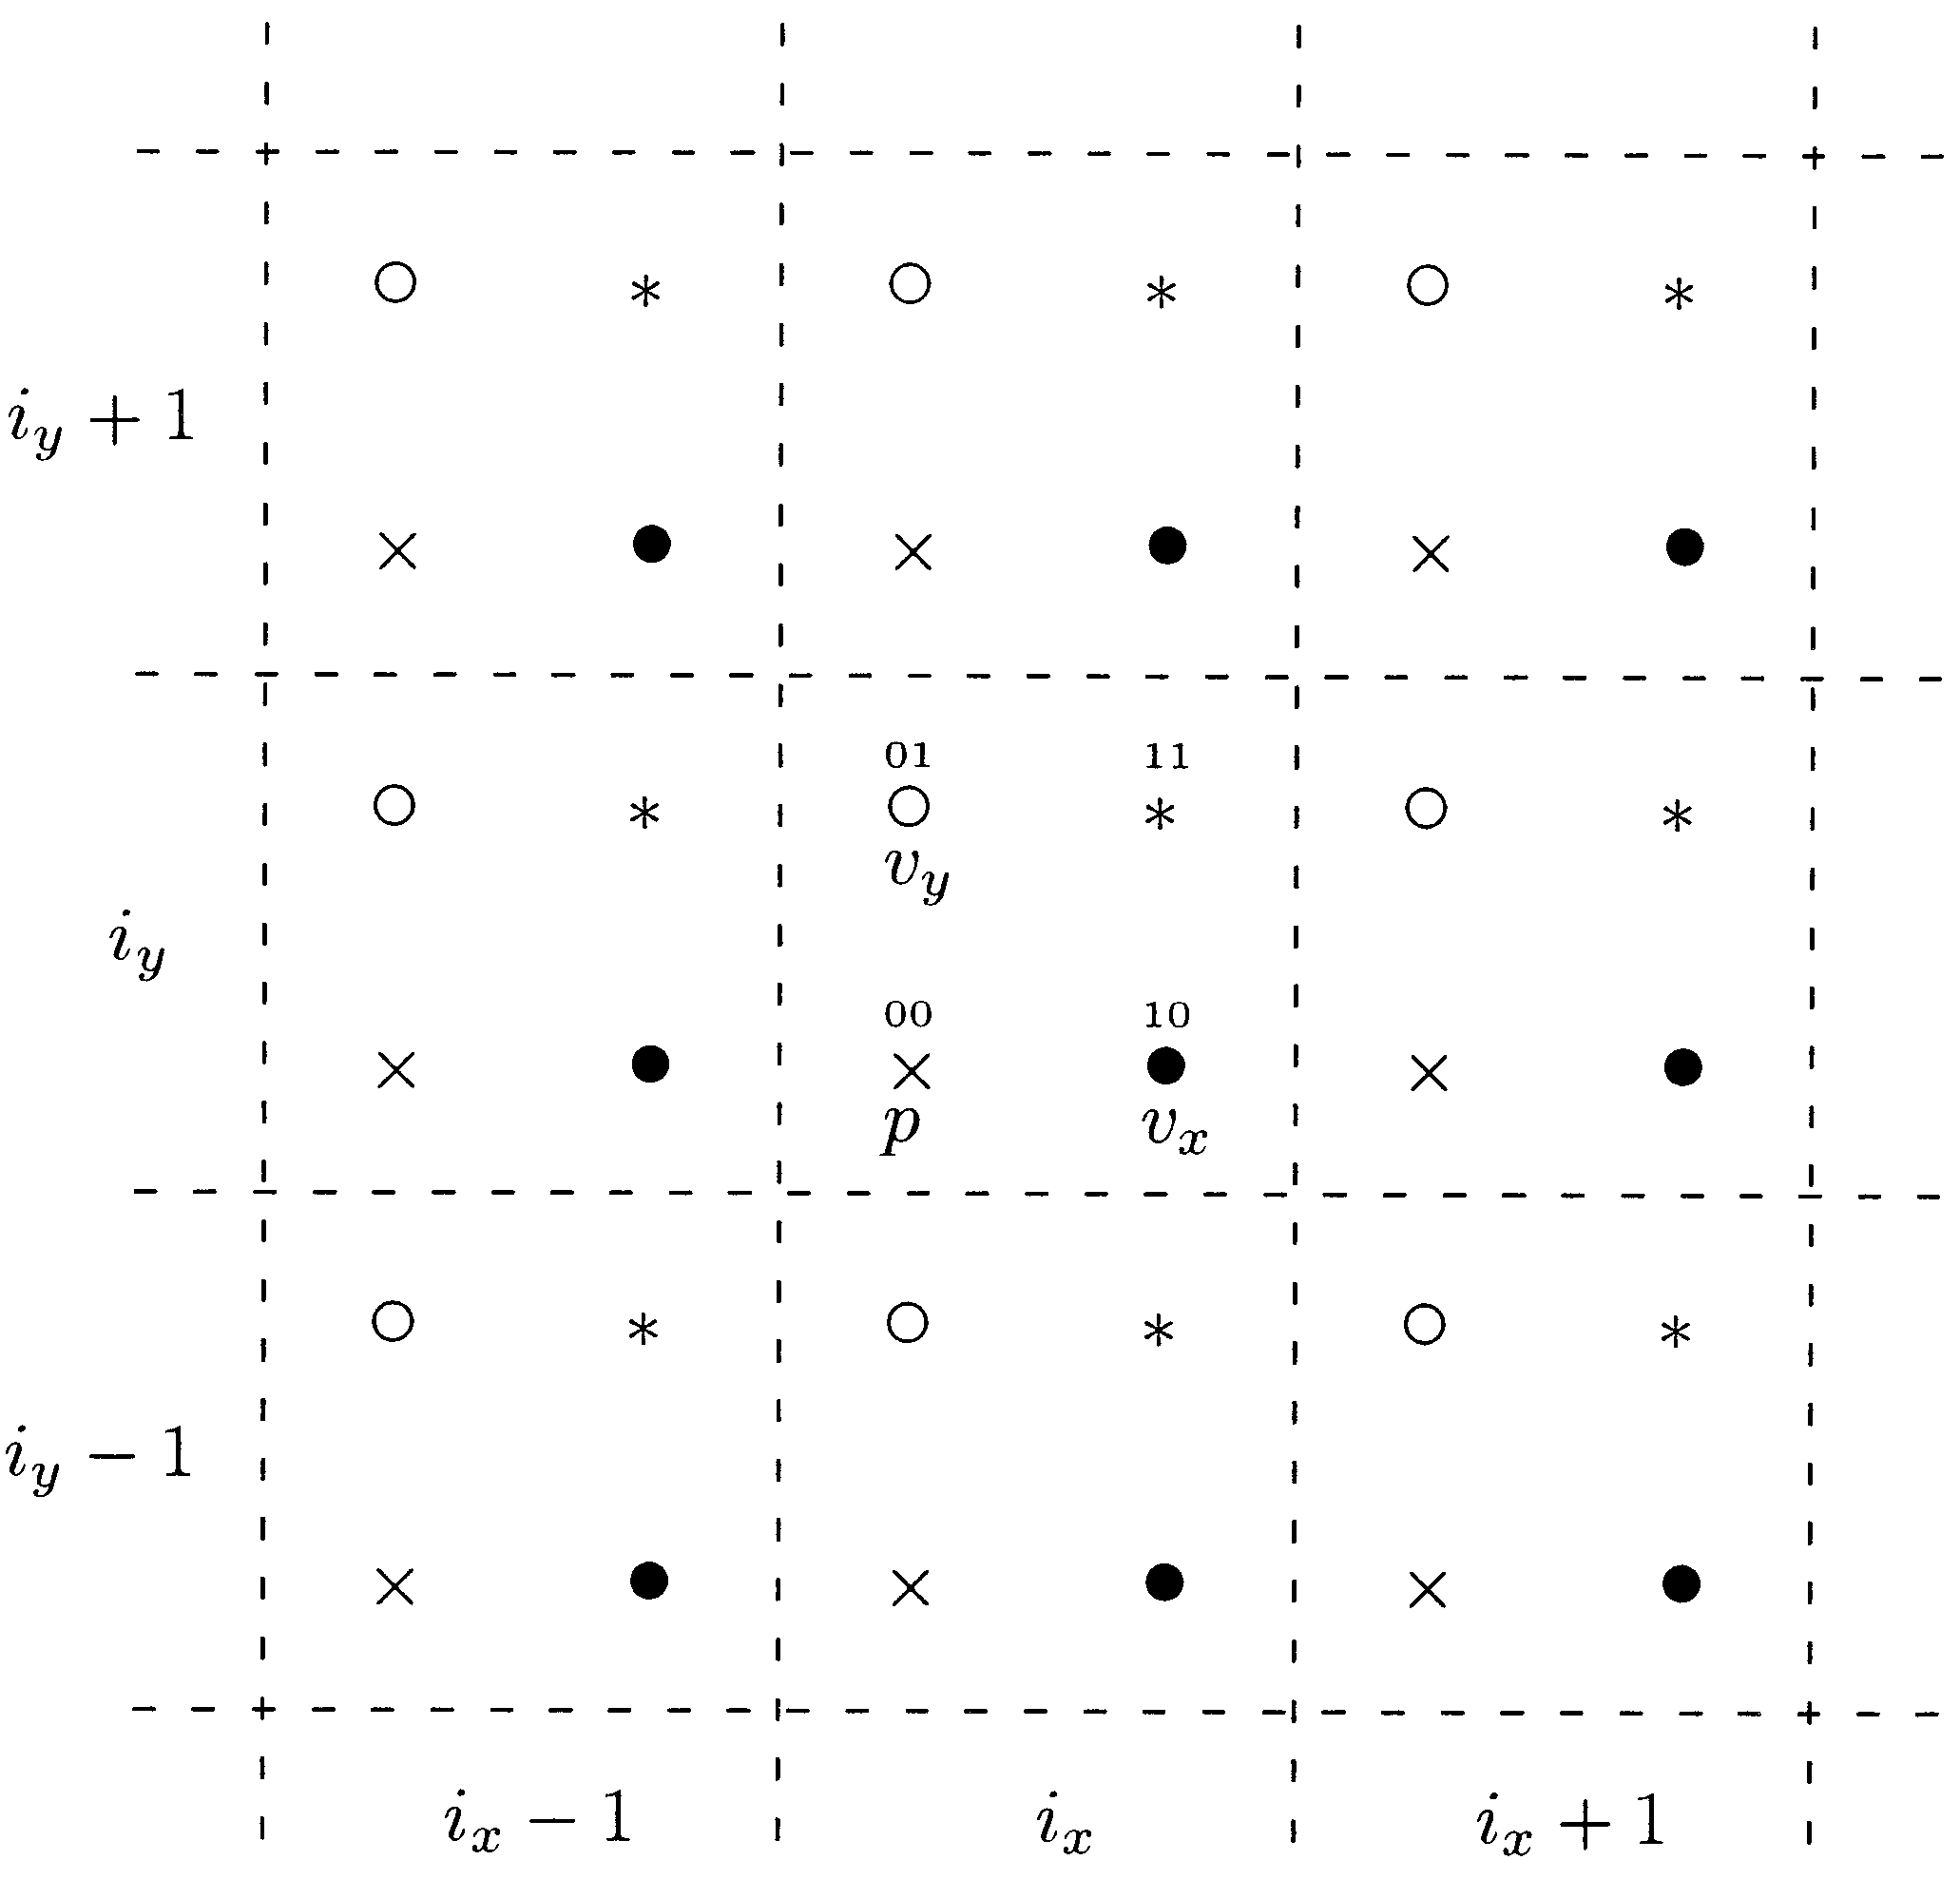
\includegraphics[width=0.4\textwidth]{figures/stag1}
	\caption{The placement of the pressure and velocity variables on a 2D staggered grid. The dashed squares denote the cells. The figure is taken form \citet{Lautrup}.}
	\label{fig:1}
\end{figure}
With this information in hand equation \eqref{o1} can be discretized as follows
\begin{equation}
	\rho \begin{bmatrix}
		\frac{v_x[i_x,i_y,i_z,t+1]-v_x[i_x,i_y,i_z,t]}{\Delta t}\\
		\frac{v_y[i_x,i_y,i_z,t+1]-v_y[i_x,i_y,i_z,t]}{\Delta t}\\
		\frac{v_z[i_x,i_y,i_z,t+1]-v_z[i_x,i_y,i_z,t]}{\Delta t}\\
	\end{bmatrix}=\begin{bmatrix}
		f_x[i_x,i_y,i_z,t]-\frac{p[i_x+1,i_y,i_z,t]-p[i_x,i_y,i_z,t]}{\Delta x}\\
		f_y[i_x,i_y,i_z,t]-\frac{p[i_x,i_y+1,i_z,t]-p[i_x,i_y,i_z,t]}{\Delta y}\\
		f_z[i_x,i_y,i_z,t]-\frac{p[i_x,i_y,i_z+1,t]-p[i_x,i_y,i_z,t]}{\Delta z}\\
	\end{bmatrix}.
\end{equation}
Note that the first equation is located on the same grid-point as $v_x$, the second on the same grid-point as $v_y$ and the third on the same grid-point as $v_z$. From the derivative of the pressure it is clear that the $v_z$ point must be orthogonal to the pressure point\footnote{$v_z$ is out of the screen on figure \ref{fig:1} since $i_z+1$ minus $i_z$ must land on the pressure point.}. This information is important since the different components of the generalized force is forced to be located on the grid-points corresponding to the rest of the given equation. Writing out the generalized force
\begin{equation}
	\vec{f}=\begin{bmatrix}
		f_{b,x}-\rho\big(v_x\frac{\partial v_x}{\partial x}+v_y\frac{\partial v_x}{\partial y}+v_z\frac{\partial v_x}{\partial z}\big)+\eta \big[\frac{\partial^2 v_x}{\partial x^2}+\frac{\partial^2 v_x}{\partial y^2}+\frac{\partial^2 v_x}{\partial z^2}+(\frac{1}{3}+\frac{\zeta}{\eta})\big(\frac{\partial^2 v_x}{\partial x^2}+\frac{\partial^2 v_y}{\partial x\partial y}+\frac{\partial^2 v_z}{\partial x\partial z}\big)\big]\\
		f_{b,y}-\rho\big(v_x\frac{\partial v_y}{\partial x}+v_y\frac{\partial v_y}{\partial y}+v_z\frac{\partial v_y}{\partial z}\big)+\eta \big[\frac{\partial^2 v_y}{\partial x^2}+\frac{\partial^2 v_y}{\partial y^2}+\frac{\partial^2 v_y}{\partial z^2}+(\frac{1}{3}+\frac{\zeta}{\eta})\big(\frac{\partial^2 v_x}{\partial y\partial x}+\frac{\partial^2 v_y}{\partial y^2}+\frac{\partial^2 v_z}{\partial y\partial z}\big)\big]\\
		f_{b,z}-\rho\big(v_x\frac{\partial v_z}{\partial x}+v_y\frac{\partial v_z}{\partial y}+v_z\frac{\partial v_z}{\partial z}\big)+\eta \big[\frac{\partial^2 v_z}{\partial x^2}+\frac{\partial^2 v_z}{\partial y^2}+\frac{\partial^2 v_z}{\partial z^2}+(\frac{1}{3}+\frac{\zeta}{\eta})\big(\frac{\partial^2 v_x}{\partial z\partial x}+\frac{\partial^2 v_y}{\partial z\partial y}+\frac{\partial^2 v_z}{\partial z^2}\big)\big]\\
	\end{bmatrix}.
\end{equation}
In order for the advective term ($\propto \rho$) to belong to the same point as $v_x$, the derivative must be averaged over the adjacent points, meaning e.g.
\begin{equation}
	\begin{split}
		&v_x\frac{\partial v_x}{\partial x} \rightarrow  v_x[i_x,i_y,i_z,t]\frac{v_x[i_x+1,i_y,i_z,t]-v_x[i_x-1,i_y,i_z,t]}{2\Delta x},\\
		&v_y\frac{\partial v_x}{\partial y}\rightarrow  \braket{v_y}\frac{v_x[i_x,i_y+1,i_z,t]-v_x[i_x,i_y-1,i_z,t]}{2\Delta y},\\
		&v_z\frac{\partial v_x}{\partial z}\rightarrow  \braket{v_z}\frac{v_x[i_x,i_y,i_z+1,t]-v_x[i_x,i_y,i_z-1,t]}{2\Delta z},\\
	\end{split}
\end{equation}
where
\begin{equation}
	\begin{split}
		&\braket{v_y}\equiv \frac{v_y[i_x,i_y,i_z,t]+v_y[i_x,i_y-1,i_z,t]+v_y[i_x+1,i_y,i_z,t]+v_y[i_x+1,i_y-1,i_z,t]}{4},\\
		&\braket{v_z}\equiv \frac{v_z[i_x,i_y,i_z,t]+v_z[i_x,i_y,i_z-1,t]+v_z[i_x,i_y+1,i_z,t]+v_z[i_x,i_y+1,i_z-1,t]}{4}.\\
	\end{split}
\end{equation}
The second derivatives are with respect to the same variable are naturally located on the same point e.g.
\begin{equation}
	\begin{split}
		&\frac{\partial^2 v_x}{\partial x^2} \rightarrow  \frac{v_x[i_x+1,i_y,i_z,t]+v_x[i_x-1,i_y,i_z,t]-2v_x[i_x,i_y,i_z,t]}{\Delta x^2},\\
		&\frac{\partial^2 v_x}{\partial y^2}\rightarrow   \frac{v_x[i_x,i_y+1,i_z,t]+v_x[i_x,i_y-1,i_z,t]-2v_x[i_x,i_y,i_z,t]}{\Delta x^2},\\
		&\frac{\partial^2 v_x}{\partial z^2}\rightarrow  \frac{v_x[i_x,i_y,i_z+1,t]+v_x[i_x,i_y,i_z-1,t]-2v_x[i_x,i_y,i_z,t]}{\Delta x^2}.\\
	\end{split}
\end{equation}
For the divergence term it is less simple for the terms with mixed derivatives. Here the average of both derivatives must be used such that
\begin{equation}
	\begin{split}
		\frac{\partial^2 v_x}{\partial x\partial y} \rightarrow \frac{1}{4\Delta x \Delta y}\bigg(&v_x[i_x+1,i_y+1,i_z,t]+v_x[i_x-1,i_y-1,i_z,t]\\
		&-v_x[i_x+1,i_y-1,i_z,t]-v_x[i_x-1,i_y+1,i_z,t]\bigg),\\
	\end{split}
\end{equation}                           
\begin{equation}
	\begin{split}
		\frac{\partial^2 v_x}{\partial x\partial z} \rightarrow \frac{1}{4\Delta x \Delta z}\bigg(&v_x[i_x+1,i_y,i_z+1,t]+v_x[i_x-1,i_y,i_z-1,t]\\
		&-v_x[i_x+1,i_y,i_z-1,t]-v_x[i_x-1,i_y,i_z-1,t]\bigg),\\
	\end{split}
\end{equation}   
The specific approach (read programming) to obtaining a solution from the discretized equations of motion depend on the physical scenario under consideration and potential simplifying assumptions that can be made.

\begin{example}
	The perhaps most used simplification of Navier-Stokes equations is to take the fluid to be incompressible ($\rho\simeq const$). Taking the density to be constant means the velocity field will be divergence-less. To see this, consider a material particle riding along with the flow in a fluid. At time $t+\delta t$ the particle will be displaced by an amount $\vec{x}+v(\vec{x},t)\delta t$. The change in mass density during this time
	\begin{equation}
		\begin{split}
			\delta \rho &=\rho(\vec{x}+v(\vec{x},t)\delta t,t+\delta t)-\rho(\vec{x},t)\\
			&= v_{x}\delta t\frac{\partial \rho (\vec{x},t)}{\partial x}+v_{y}\delta t\frac{\partial \rho (\vec{x},t)}{\partial y}+v_{z}\delta t\frac{\partial \rho (\vec{x},t)}{\partial z}+\delta t\frac{\partial \rho (\vec{x},t)}{\partial t}+\mathcal{O}(\delta t^2)\\
			&=\bigg(\frac{\partial \rho}{\partial t}+(\vec{v}\cdot \vec{\nabla})\rho\bigg)\delta t.
		\end{split}
	\end{equation}
	Dividing by $\delta t$ reveals the rate of change of density as seen from the material particle, i.e. the material derivative of the density
	\begin{equation}
		\frac{D \rho}{Dt}=\frac{\partial \rho}{\partial t}+(\vec{v}\cdot \vec{\nabla})\rho.
		\label{one}
	\end{equation}
	Imposing conservation of mass means
	\begin{equation}
		\frac{\partial \rho}{\partial t}+\vec{\nabla}(\rho\vec{v})=0,
		\label{two}
	\end{equation}
	with $\vec{\nabla}(\rho\vec{v})=(\vec{v}\cdot \vec{\nabla})\rho+\rho\vec{\nabla}\cdot \vec{v}$. Combining equation \eqref{one} and \eqref{two} reveals
	\begin{equation}
		\frac{D \rho}{Dt}+\rho\vec{\nabla}\cdot \vec{v}=0.
		\label{three}
	\end{equation}
	From equations \eqref{three} and \eqref{one} it is clear that by taking $\rho=const$ the material derivative vanish and by extension it is required that the velocity field is divergence-free ($\vec{\nabla}\cdot \vec{v}=0$). This information can be used to simplify the Navier-Stokes equations. Taking the divergence of equation \eqref{o1}
	\begin{equation}
		\vec{\nabla}^2p=\vec{\nabla}\cdot\vec{f}\equiv s,
		\label{o3}
	\end{equation}
	where $s$ abbreviates "source". 
\end{example}



\chapter{Analytical Mechanics}
Analytical mechanics, derived primarily by Joseph-Louis Lagrange and William Rowan Hamilton in the late 1700's and early 1800's, is a framework equivalent to Newtonian mechanics for conservative forces\footnote{The Lagrangian formalism utilizes the potential energy function which is only defined for a conservative force field. Non-conservative forces can be incorporated with much difficulty however.}. The framework consists of three equivalent schemes; Lagrangian mechanics, Hamiltonian mechanics and Hamilton-Jacobi mechanics. These schemes provide the foundation for three of the quantum mechanical formalisms. These generalizations will be considered in chapter \ref{chp:4}. 
\begin{figure}[h]
	\captionsetup{width=1\textwidth}
	\centering
	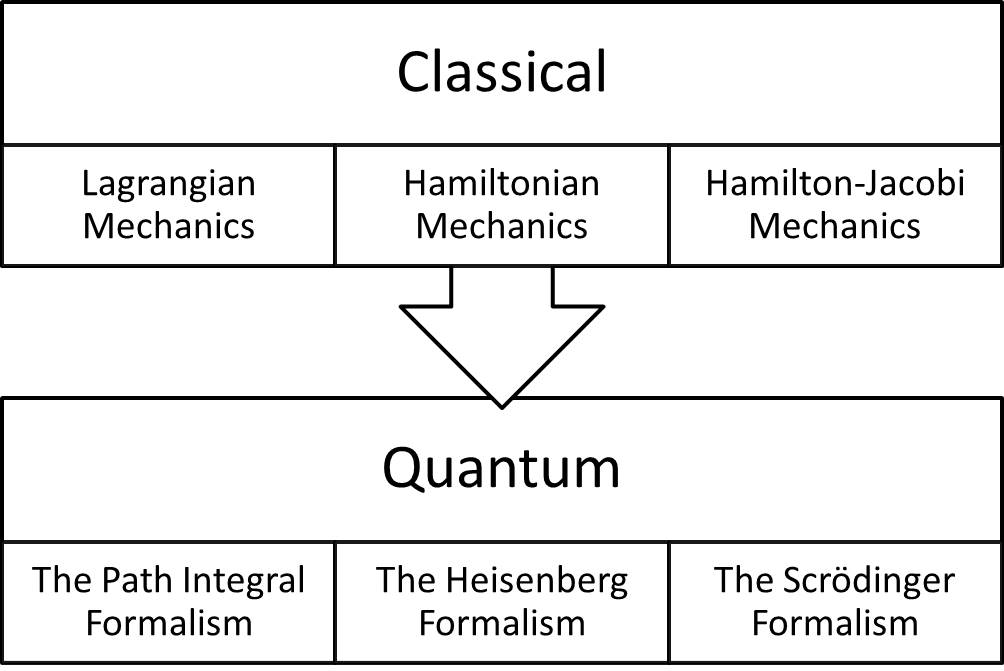
\includegraphics[width=0.5\textwidth]{figures/Billede1}
\end{figure}
The schemes of analytical mechanics was derived with the intention to investigate the fundamental processes in nature that led to Newtons laws. This quest was by and large successful and significant physical insight can be gained by studying the schemes of analytical mechanics. 

\section{Lagrangian Mechanics}
The Lagrangian formalism was introduced by Joseph-Luis Lagrange in 1788 ($\sim100$ years after Newtons laws). Back in the days scientists were concentrated on finding a more general formulation of the principles of physics - Compared to the Newtonian formalism. Newtons laws provide instructions to acquire the laws of motion, but they do not provide an explanation as to \emph{why} the laws are in the way they are. An explanation as to why came from developing Lagrangian mechanics; everything in physics derives from the principle of least action! 

\subsection*{The principle of least action}
Consider a generic physical system which has an instantaneous configuration described by the values of $n$ generalized coordinates, $\bar{q}\equiv(q_1, q_2,...q_n)$. Because the generalized coordinates determine the configuration of the system, they span what is called \emph{configuration space}\index{Configuration space}, and the physical state of the system is given as a point in this $n$-dimensional hyperspace~\citep{Goldstein}. As time progresses, the state of the general physical system will change. For the generalized coordinates, this change of state results in the point tracing out a line (or path), called the path of motion, in configuration space. Which path of motion the system will take is described by \emph{Hamiltons principle}\index{Hamiltons principle}\index{Principle of least action}, also called the principle of stationary (or least) action. 

\paragraph{The principle of stationary action:} \emph{The motion of the system from time $t_1$ to $t_2$ is such that the action ($S$) is extremized (minimized most often)\footnote{The reason why the system traces the path in configuration space that corresponds to the minimized action can be explained from quantum mechanics and the path integral scheme. In the path integral scheme the transition probability is given in terms of the path integral of $e^{\frac{iS}{\hbar}}$ (SI units). In the classical limit ($\hbar\Rightarrow 0$ the exponential will fluctuate wildly and all contributions besides those which corresponds to a minimized action will cancel cf. the random phase principle.)}}\newline

The action\index{Action, classical} is defined by the integral~\citep{Sannino}
\begin{equation}
	S\big[\bar{q},\dot{\bar{q}}, t_1,t_2\big]=\int_{t_1}^{t_2}L\big(\bar{q}(t),\dot{\bar{q}}(t),t\big)dt,
	\label{action}
\end{equation} 
where the square brackets indicate that the action is a \emph{functional} rather than a \emph{function}\footnote{A function is a rule that assigns a unique element, $f(x)$, from a set to each value, $x$, in another set; a function takes in a number and produces a number. A functional, on the other hand, associates a vector valued function with a real number.}. The function $L$ is the \emph{Lagrangian}\index{Lagrangian, definition} and is defined as
\begin{equation}
	L\big(\bar{q}(t),\dot{\bar{q}}(t),t\big)=T\big(\dot{\bar{q}}(t)\big)-V\big(\bar{q}(t),t\big),
	\label{Lagrangeian}
\end{equation} 
where $T$ is the kinetic energy of the system and $V$ is the potential energy of the system. 

\subsubsection*{The Euler-Lagrange equation}
By minimizing the action of equation \eqref{action} the master equation of Lagrangian mechanics, the Euler-Lagrange equation, is obtained. Consider a variation of the action:
\begin{equation}
	\begin{split}
		\delta S\big[\bar{q},\dot{\bar{q}}, t_1,t_2\big]
		&=\delta\int_{t_1}^{t_2} L\big(\bar{q}(t),\dot{\bar{q}}(t),t\big)dt\\
		&=\int_{t_1}^{t_2}\sum_{j=1}^{n}\bigg(\frac{\partial L\big(\bar{q}(t),\dot{\bar{q}}(t),t\big)}{\partial q_j(t)}\delta q_j(t)+\frac{\partial L\big(\bar{q}(t),\dot{\bar{q}}(t),t\big)}{\partial \dot{q}_j(t)}\delta \dot{q}_j(t)\bigg)dt\\
		&=\int\sum_{j}\frac{\partial L\big(\bar{q}(t),\dot{\bar{q}}(t),t\big)}{\partial q_j(t)}\delta q_j(t)dt+\int\sum_{j}\frac{\partial L\big(\bar{q}(t),\dot{\bar{q}}(t),t\big)}{\partial \dot{q}_j(t)}\delta \dot{q}_j(t)dt,
	\end{split}
	\label{lag3}
\end{equation} 
where $\dot{\bar{q}}(t)=(\dot{q}_1(t), \dot{q}_2(t),\dots\dot{q}_n(t))$\normalsize and $\bar{q}(t)=(q_1(t), q_2(t),\dots q_n(t))$\normalsize. The last term is evaluated by partial integration
\begin{equation}
	\begin{split}
		\int\sum_{j}\frac{\partial L\big(\bar{q}(t),\dot{\bar{q}}(t),t\big)}{\partial \dot{q}_j(t)}\delta \dot{q}_j(t)dt&=\int\sum_{j}\frac{d}{dt}\bigg(\frac{\partial L\big(\bar{q}(t),\dot{\bar{q}}(t),t\big)}{\partial \dot{q}_j(t)}\delta q_j(t)\bigg)dt\\
		&\quad-\int\sum_{j}\frac{d}{dt}\bigg(\frac{\partial L\big(\bar{q}(t),\dot{\bar{q}}(t),t\big)}{\partial \dot{q}_j(t)}\bigg)\delta q_j(t)dt,
	\end{split}
	\label{lag2}
\end{equation} 
where
\begin{equation}
	\int_{t_1}^{t_2}\sum_{j}\frac{d}{dt}\bigg(\frac{\partial L\big(\bar{q}(t),\dot{\bar{q}}(t),t\big)}{\partial \dot{q}_j(t)}\delta q_j(t)\bigg)dt=\sum_{j}\frac{\partial L\big(\bar{q}(t),\dot{\bar{q}}(t),t\big)}{\partial \dot{q}_j(t)}\delta q_j(t)\bigg|_{t_1}^{t_2}=0.
	\label{lag1}
\end{equation} 
Equation \eqref{lag1} vanish by taking the endpoints of the path to be fixed, i.e. $\delta q_j(t_1)=\delta q_j(t_2)=0$ is taken as boundary conditions. By using equation \eqref{lag1} in equation \eqref{lag2} and the result in equation \eqref{lag3} the variation in the action can be written as
\begin{equation}
	\delta S\big[\bar{q},\dot{\bar{q}}, t_1,t_2\big]=\int\sum_{j}\bigg(\frac{\partial L\big(\bar{q}(t),\dot{\bar{q}}(t),t\big)}{\partial q_j(t)}-\frac{d}{dt}\bigg(\frac{\partial L\big(\bar{q}(t),\dot{\bar{q}}(t),t\big)}{\partial \dot{q}_j(t)}\bigg) \bigg)\delta q_j(t)dt.
	\label{lag4}
\end{equation} 
To minimize the action (find a minimum in $S$), the variation (equation \eqref{lag4}) must vanish. In order for the variation to vanish for an arbitrary $\delta q_j(t)$, the remaining part of the integrand must always be zero. That is
\begin{equation}
	\frac{\partial L\big(\bar{q}(t),\dot{\bar{q}}(t),t\big)}{\partial q_j(t)}-\frac{d}{dt}\bigg(\frac{\partial L\big(\bar{q}(t),\dot{\bar{q}}(t),t\big)}{\partial \dot{q}_j(t)}\bigg)=0. 
	\label{lag5}
\end{equation} 
Equation \eqref{lag5} is called the \emph{Euler-Lagrange} equation\index{Euler-Lagrange equation}. It is often written in the less detailed form
\begin{equation}
	\frac{\partial L}{\partial q_j}-\frac{d}{dt}\bigg(\frac{\partial L}{\partial \dot{q}_j}\bigg)=0. 
	\label{EL}
\end{equation} 
The Euler-Lagrange equation is a second order differential equation in time, and from it the equations of motion can be determined by specifying, and inserting, the Lagrangian. Thus, the Euler-Lagrange equation is equivalent to Newtonian dynamics, but instead of postulating a series of laws, the equations of motions are derived from the assumption that the path of the system in configuration space is the path of least action. This provides profound, new physical insight into the machinery of nature.
\begin{example}
	\emph{Determine and solve the EOM for a movable, simple pendulum.}\newline
	
	The movable, simple pendulum consist of two particles; one particle ($m_1$) is confined to a horizontal movement, whereas another particle ($m_2$) is attached to the first via a (massless) string, and is free to swing back and forth - See figure \ref{fig:sphere}.
	\begin{figure}[h]
		\captionsetup{width=1\textwidth}
		\centering
		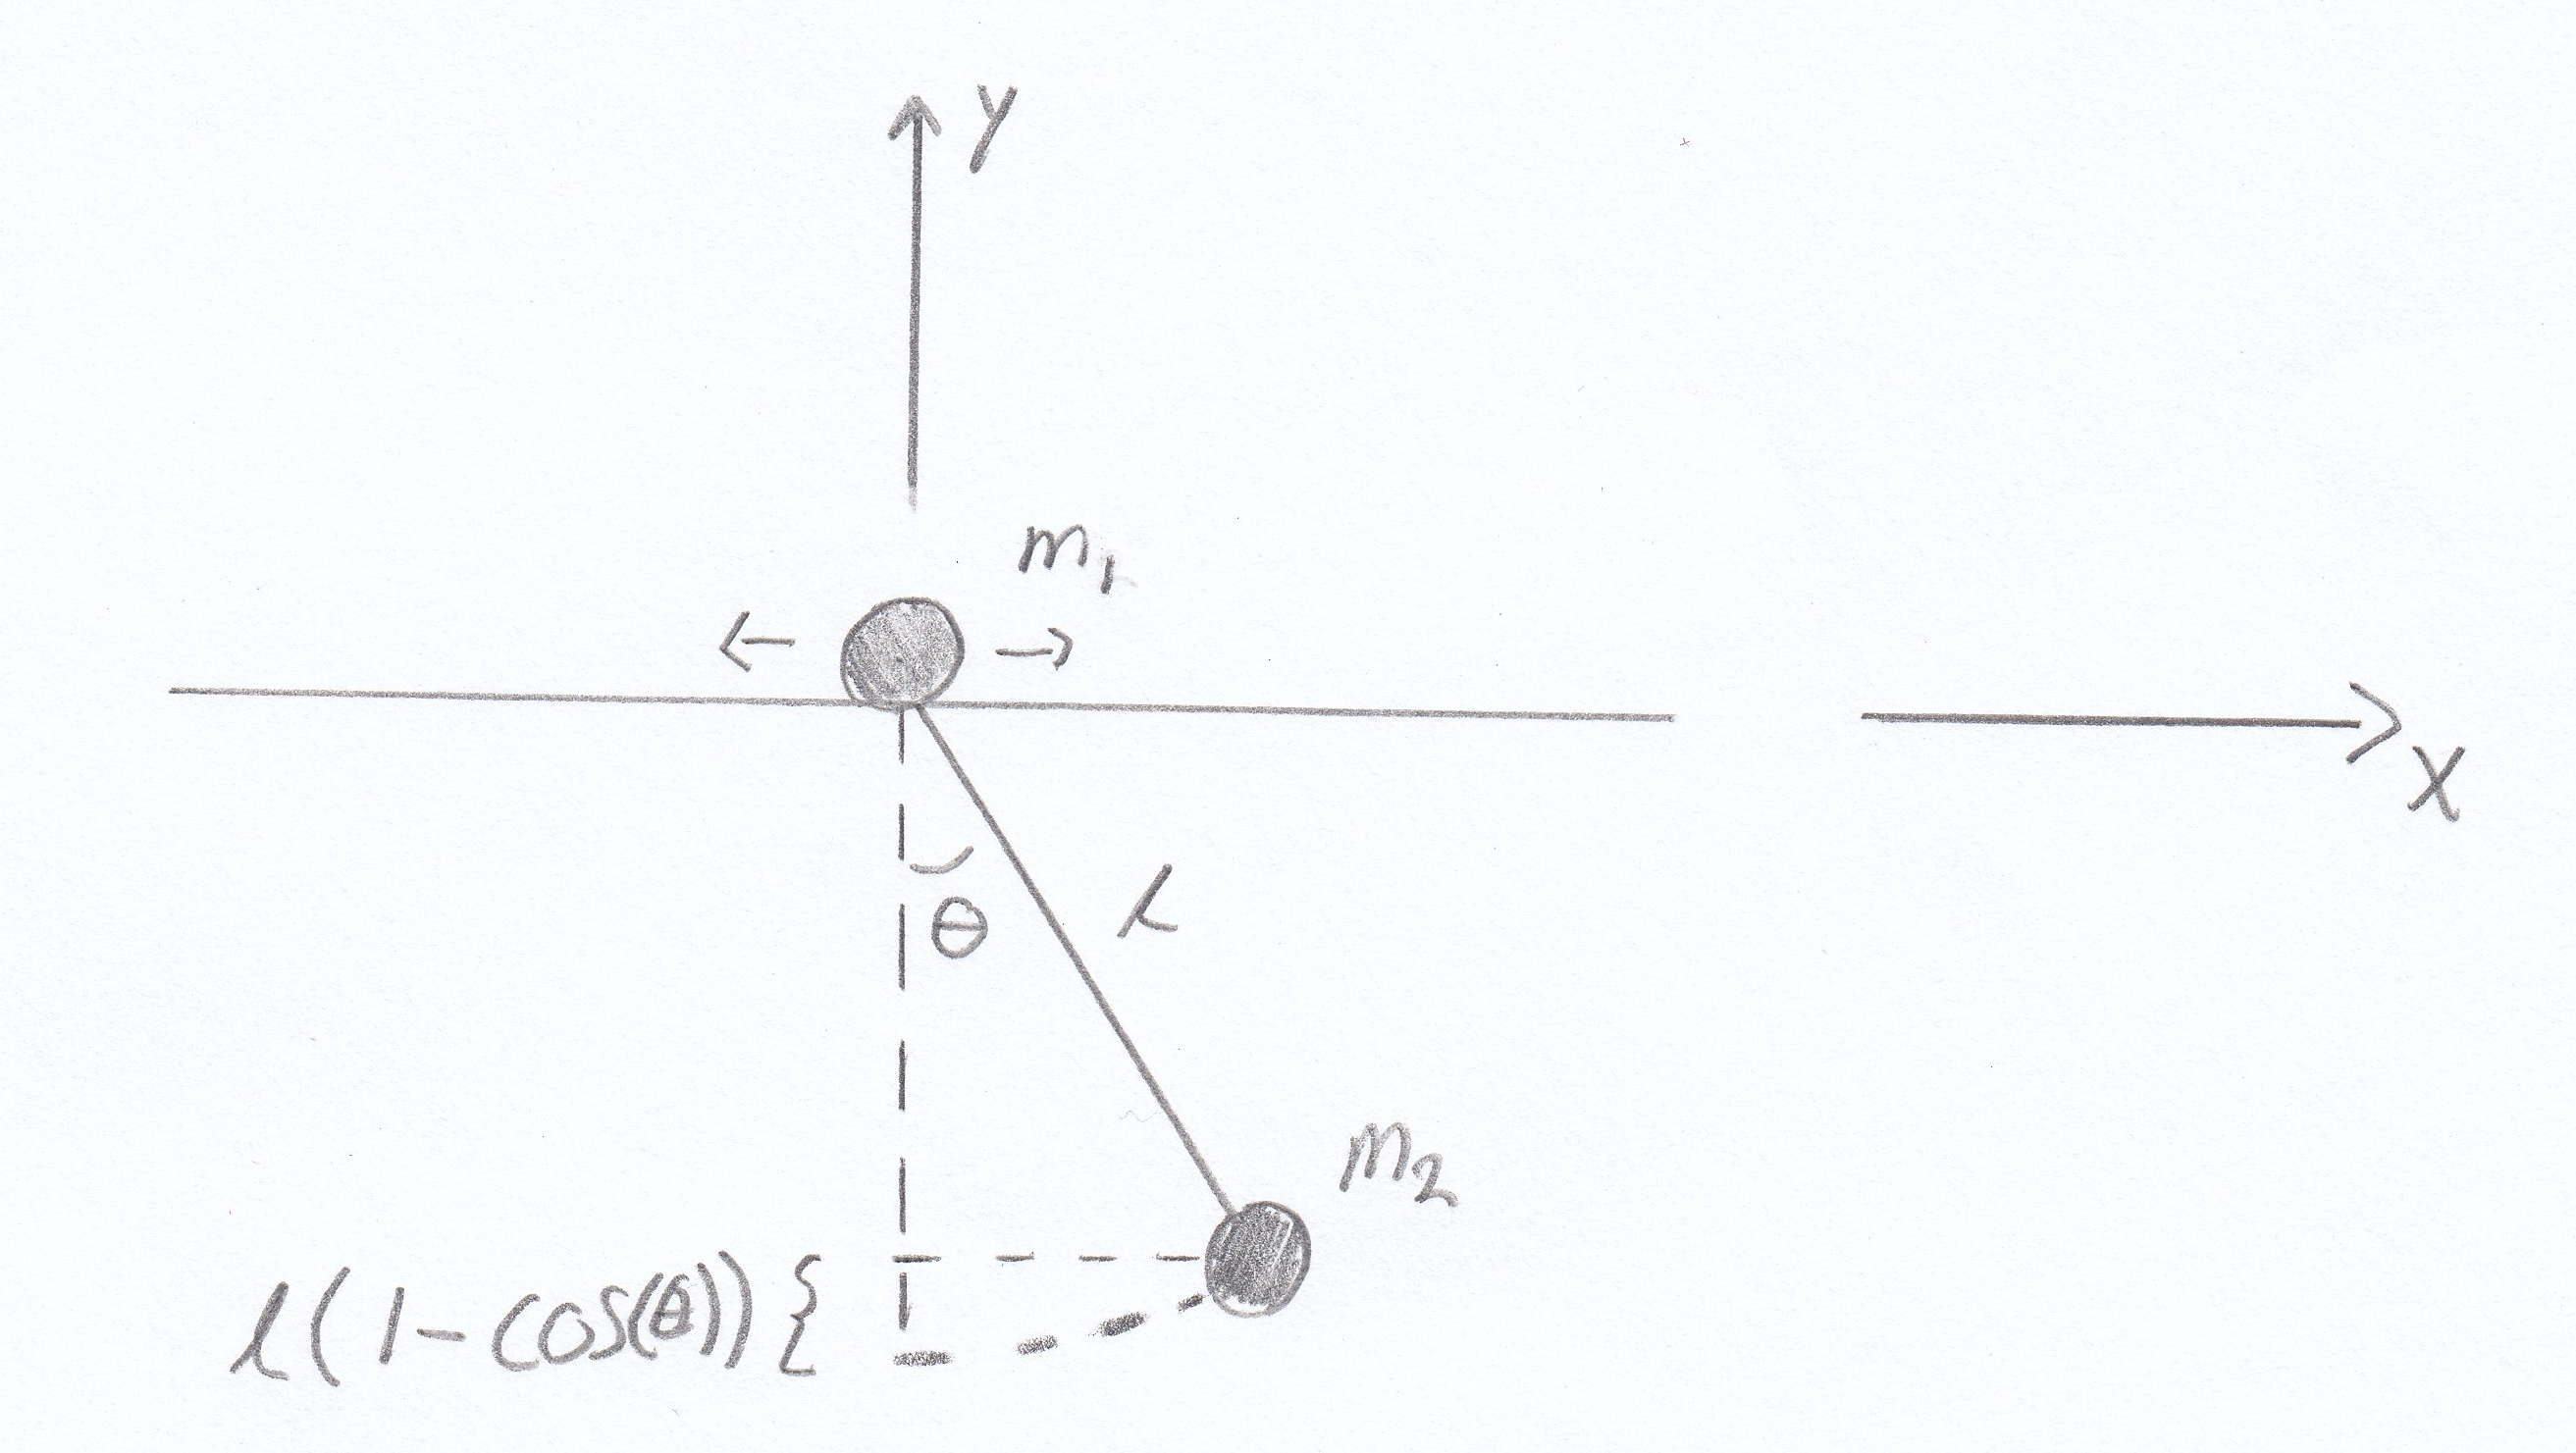
\includegraphics[width=0.5\textwidth]{figures/sphere}
		\caption{The spherical pendulum with spherical coordinates.}
		\label{fig:sphere}
	\end{figure}
	In terms of the, from the figure, defined coordinate system, the coordinates are given by
	\begin{equation}
		x_1=x_1, \quad y_1=0,
	\end{equation} 
	\begin{equation}
		x_2=x_1+lsin(\theta), \quad y_2=-lcos(\theta),
	\end{equation} 
	where the minus sign in $y_2$ is there because the second particle is defined to swing at negative $y$. For the potential energy in the Lagrangian the relevant distance\footnote{So that the potential energy is positive when the mass is displaced from equilibrium.} is the vertical displacement from equilibrium $(l-y_2)$, so the Lagrangian is given by
	\begin{equation}
		L=\frac{1}{2}m_1\dot{x}_1^2+\frac{1}{2}m_2(\dot{x}_2^2+\dot{y}_2^2)-m_2gl(1-cos(\theta)).
	\end{equation} 
	The velocity of the second particle is
	\begin{equation}
		\begin{split}
			\dot{x}_2^2+\dot{y}_2^2&=\dot{x}_1^2+2\dot{x}_1lcos(\theta)\dot{\theta}+l^2cos(\theta)^2\dot{\theta}^2+l^2sin(\theta)^2\dot{\theta}^2\\
			&=\dot{x}_1^2+l^2\dot{\theta}^2+2l\dot{x}_1\dot{\theta}cos(\theta).
		\end{split}
	\end{equation} 
	So
	\begin{equation}
		L=\frac{1}{2}m_1\dot{x}_1^2+\frac{1}{2}m_2(\dot{x}_1^2+l^2\dot{\theta}^2+2l\dot{x}_1\dot{\theta}cos(\theta))-m_2gl(1-cos(\theta)).
	\end{equation} 
	Using $x_1$ and $\theta$ as generalized coordinates, the EOM can be found from the Euler-Lagrange equation
	\begin{equation}
		\underbrace{\frac{\partial L}{\partial x_1}}_{=0}-\frac{d}{dt}\bigg(\frac{\partial L}{\partial \dot{x}_1}\bigg)=0\Rightarrow \dot{x}_1(m_1+m_2)+m_2lcos(\theta)\dot{\theta}=const=p_{x_1},
	\end{equation} 
	\begin{equation}
		\begin{split}
			0&=\frac{\partial L}{\partial \theta}-\frac{d}{dt}\bigg(\frac{\partial L}{\partial \dot{\theta}}\bigg)\Rightarrow -m_2lsin(\theta)(\dot{x}_1\dot{\theta}+g)-m_2l(l\ddot{\theta}+\ddot{x}_1cos(\theta)-\dot{x}_1\dot{\theta}sin(\theta))=0.
		\end{split}
	\end{equation} 
	Two of the terms ($\dot{x}_1\dot{\theta}$) cancel, so
	\begin{equation}
		m_2l^2\ddot{\theta}+m_2glsin(\theta)+m_2l\ddot{x}_1cos(\theta)=0.
	\end{equation} 
	Eliminate $\ddot{x}_1$ from the above equation by using the Euler-Lagrange equation for $x_1$. Hereby
	\begin{equation}
		\begin{split}
			0&=\ddot{x}_1(m_1+m_2)+m_2l(cos(\theta)\ddot{\theta}-sin(\theta)\dot{ \theta}^2)\\
			&\Rightarrow \ddot{x}_1=\frac{m_2l}{m_1+m_2}(\dot{\theta}^2sin(\theta)-\ddot{\theta}cos(\theta)).
		\end{split}
	\end{equation} 
	So
	\begin{equation}
		m_2l^2\ddot{\theta}-\frac{m_2^2l^2cos(\theta)^2}{m_1+m_2}\ddot{\theta}+\frac{m_2^2l^2cos(\theta)sin(\theta)}{m_1+m_2}\dot{\theta}^2+m_2lgsin(\theta)=0.
	\end{equation} 
	This is in general difficult to solve, so I consider the  limiting cases
	\begin{equation}
		m_2\gg m_1 \wedge \theta=\text{small:}\quad \dot{\theta}^2+\frac{g}{l}\approx 0 \Rightarrow \theta\approx
		\sqrt{-\frac{g}{l}}t+A.
	\end{equation} 
	Since $g>0$ the above EOM is complex. This makes sense physically since if $m_2\gg m_1$, $m_2$ will drag $m_1$ along and no swinging motion at small angles will occur. Hence, $m_2\gg m_1$ and $\theta=\text{small}$ ar incompatible approximations. Instead I consider $m_2\ll m_1 \wedge \theta=\text{small}$. This corresponds to a small mass swinging fro a large mass. In the limit of large $m_1$ this should simplify to the simple pendulum since at small angles $m_1$ should not move. Indeed this is what I find
	\begin{equation}
		m_2\ll m_1 \wedge \theta=\text{small:}\quad \ddot{\theta}+\frac{g}{l}\theta\approx 0 \Rightarrow \theta\approx \theta_0cos\bigg(\sqrt{\frac{g}{l}}t\bigg).
	\end{equation} 
\end{example}
Since the equations of motion falls out directly from the Euler-Lagrange equation, and since the equations of motion in Newtonian mechanics are directly related to the rate of change of momentum, it is no surprise that the momentum, and the rate of change of momentum, is related to the Euler-Lagrange equation. However, since the Euler-Lagrange equation deals with generalized coordinates, the momentum that is referred to is not necessarily the linear momentum. If for example a system of polar coordinates are considered, the momentum derived from the Euler-Lagrange equation is the angular momentum. Thus, the momentum related to the Euler-Lagrange equation is called the canonical momentum conjugate \index{Conjugate momentum} to the generalized coordinate $q_j$, $p_j$, and it is defined as
\begin{equation}
	p_j=\frac{\partial L}{\partial \dot{q}_j}.
	\label{conj. momentum}
\end{equation} 
By using this definition in the Euler-Lagrange-equation, it directly follows that
\begin{equation}
	\dot{p}_j=\frac{\partial L}{\partial q_j}.
	\label{diff. conj. momentum}
\end{equation} 
Using equation \eqref{conj. momentum} and \eqref{diff. conj. momentum} in the Euler-Lagrange equation it is clear that it (the Euler-Lagrange equation) stipulates $\dot{p}-\dot{p}=0$, which is indeed the case. Memo-technically this is a good thing to remember because one of the quantities are to be differentiated wrt. time, so if the equation must read $\dot{p}-\dot{p}=0$ it can be deduced that $\frac{\partial L}{\partial \dot{q}_j}$, which is to be differentiated wrt. time in the Euler-Lagrange equation, must equal $p$. From equation \eqref{diff. conj. momentum} it follows that if the Lagrangian does not depend on a given coordinate, $q_j$, the corresponding momentum is conserved; $\frac{\partial p_j}{\partial t}=0\Rightarrow p_j=\mbox{conserved}$. An alternative way to formulate the principle of conserved quantities is via Noethers theorem\index{Noethers theorem, classical mechanics}.

\paragraph{Noethers theorem:}\emph{Transformations under which the Lagrangian is unchanged have a conserved quantity associated to them.}


\begin{example}
	Consider a translational invariant physical system described by the Lagrangian $L(x_i,\dot{x}_i)$. A constant displacement of $x_i$ will leave the Lagrangian invariant. Hence, the Lagrangian is invariant under the transformation
	\begin{equation}
		x_i\Rightarrow x_i+\delta x,
	\end{equation} 
	where $\delta x$ is a constant. The change in the Lagrangian under this transformation can be described as
	\begin{equation}
		\delta L=\frac{\partial L}{\partial x_i}\delta x_i+\frac{\partial L}{\partial \dot{x}_i}\delta\dot{x}_i=\delta x\frac{\partial L}{\partial x_i}=\delta x\frac{d}{dt}\bigg(\frac{\partial L}{\partial \dot{x}_i}\bigg)=0,
	\end{equation} 
	where $\delta L=0$ cf. the invariance of $L$ under the transformation and the Euler-Lagrange equation has been used for the last equality. Since $\delta x\neq0$ in general, $\frac{d}{dt}\big(\frac{\partial L}{\partial \dot{x}_i}\big)=0$ must hold and so $\frac{\partial L}{\partial \dot{x}_i}=p_i=const$ w.r.t. time. This example therefore illustrates how invariance of the Lagrangian, under a constant spatial translation, leads to conservation of linear momentum. 
\end{example}

\begin{example}
	Consider a Lagrangian that is invariant under the infinitesimal rotation around some vector, $\delta \vec{\phi}(=\epsilon \hat{n})$ i.e. the Lagrangian that is invariant under
	\begin{equation}
		\delta x_i=(\delta \vec{\phi} \times \vec{r})_i,
	\end{equation} 
	where $\vec{r}$ is the radius vector in spherical coordinates. Then change in the Lagrangian under this transformation can be described viz
	\begin{equation}
		\begin{split}
			\delta L&=\frac{\partial L}{\partial x_i}\delta x_i+\frac{\partial L}{\partial \dot{x}_i}\delta\dot{x}_i\\
			&=\frac{\partial L}{\partial x_i}(\delta \vec{\phi} \times \vec{r})_i+\frac{\partial L}{\partial \dot{x}_i}(\delta \vec{\phi} \times \dot{\vec{r}})_i\\
			&=\dot{\vec{p}}\cdot(\delta \vec{\phi} \times \vec{r})+\vec{p}\cdot(\delta \vec{\phi} \times \dot{\vec{r}})\\
			&=\delta \vec{\phi}\cdot[(\vec{r}\times\dot{\vec{p}})+(\dot{\vec{r}}\times\vec{p})]\\
			&=\delta\vec{\phi}\cdot\frac{d}{dt}\bigg(\vec{r}\times\vec{p}\bigg)=0.\\
		\end{split}
	\end{equation} 
	Since $\delta \vec{\phi}\neq \vec{0}$ in general; $\frac{d}{dt}\big(\vec{r}\times\vec{p}\big)=\vec{0}$ must hold and so $\vec{L}=\vec{r}\times\vec{p}=const$. This example illustrates how invariance of the Lagrangian, under a constant spatial rotation, leads to conservation of angular momentum.
	
\end{example}

\begin{example}
	\emph{Consider the transformation $q\Rightarrow q+\epsilon$, where $\epsilon$ is an infinitesimal, constant parameter. Why does this transformation not change the EOM?}\newline
	
	Invariance in the EOM means $\delta S=\delta S'=0$, where $S$ and $S'$ refers to the action before and after transformation. To show that this is indeed the case, consider the Taylor expansion of the transformed Lagrangian
	\begin{equation}
		\begin{split}
			L(q+\epsilon,\dot{q})&=L(q,\dot{q})+\frac{\partial L}{\partial q}\epsilon+\mathcal{O}(\epsilon^2)\\
			&=L(q,\dot{q})+\dot{p}\epsilon,
		\end{split}
	\end{equation} 
	where equation \eqref{conj. momentum} has been used for the second equality and $\mathcal{O}(\epsilon^2)$ has been neglected since $\epsilon$ is infinitesimal. The corresponding action is given by
	\begin{equation}
		\begin{split}
			S'&=\int dt L(q+\epsilon,\dot{q})\\
			&=\int dt L(q,\dot{q})+\int dt\dot{p}\epsilon\\
			&=S+\epsilon \bigg(p(q_t,t_2)-p(q_1,t_1)\bigg).
		\end{split}
	\end{equation} 
	$S$ and $S'$ differs by a quantity which depends on the endpoints of the path. Since the path endpoints are kept fixed, this vanishes upon variation. Therefore $\delta S=\delta S'=0$. 
\end{example}
The result of example 3.2 can be generalized as follows; it is in general true that Lagrangians, which differ by a time-derivative of a function of coordinates and time, leads to the same EOM. Consider
\begin{equation}
	L'(q,\dot{q},t)=L(q,\dot{q},t)+\frac{df(q,t)}{dt},
\end{equation} 
where $f$ is a generic function of the coordinates and time. In general $L$ and $L'$ will lead to the same EOM since $\delta S=\delta S'=0$ cf. the above arguments. Therefore the Lagrangian is only defined up to a total derivative of some generic function of the coordinates and time. 

\section{Hamiltonian Mechanics}
The Lagrangian is a function of the generalized coordinates which defines a point in configuration space. Time evolution of the system traces out a path in configuration space. However, the state of the system is defined by $\{q_i\}$ and $\{p_i\}$ in the sense that this information enables a determination of the system state at all times in the future. The pair $\{q_i,p_i\}$ defines a point in $2n$-dimensional \emph{phase space}\footnote{Since a point in phase space is sufficient to determine the future evolution of the system, paths in phase space can never cross. We say that evolution is governed by a flow in phase space. The movement in phase space can therefore be modeled as the flow of an ideal (incompressible) fluid.}. The desire is therefore to find the function (the Hamiltonian) on phase space that will determine the unique evolution of $\{q_i\}$ and $\{p_i\}$ and contain the same information as the Lagrangian. Since $\{q_i,p_i\}$ and $\{q_i,\dot{q}_i\}$ are conjugate sets of variables, the Hamiltonian can be determined from the Lagrangian via a transformation called a \emph{Legendre transformation}\index{Legendre transformation}. A Legendre transformation converts a function of a set of variables to another, conjugate, set of variables. The Legendre transformation from $L\Rightarrow H$ is done in the following way; take $L=L(q_i,\dot{q}_i)$. Hereby
\begin{equation}
	\begin{split}
		dL&=\sum_i\frac{\partial L}{\partial q_i}dq_i+\sum_i\frac{\partial L}{\partial \dot{q}_i}d\dot{q}_i\\
		&=\sum_i\dot{p}_idq_i+\sum_ip_id\dot{q}_i.
	\end{split}
\end{equation} 
The variables of the function is expressed as differentials. In order to shift from $(q_i,\dot{q}_i)\Rightarrow (q_i,p_i)$ use that $\sum_ip_id\dot{q}_i=d(\sum_ip_i\dot{q}_i)-\sum_i\dot{q}_idp_i$, take the differential $d(\sum_ip_i\dot{q}_i)$ to the left hand side and reverse the signs. Hereby
\begin{equation}
	\begin{split}
		dH(q_i,p_q)&\equiv d(\sum_ip_i\dot{q}_i-L)\\
		&=-\sum_i\dot{p}_idq_i+\sum_i\dot{q}_idp_i.\\
	\end{split}
	\label{ham}
\end{equation} 
To interpret the Hamiltonian; rewrite the Hamiltonian by identifying the sum as $\sum_{j=1}^{n}\big(p_j\dot{q}_j\big)=2T$ and using that $L\equiv T-V$, the Hamiltonian can be written as\index{Hamiltonian, definition}
\begin{equation}
	H=T+V.
\end{equation} 
Hence, the Hamiltonian can be interpreted as the total energy of the system. The partial derivatives of the Hamiltonian are the Hamilton equations
\begin{equation}
	\frac{\partial H}{\partial p_i}=\dot{q}_i, \quad \frac{\partial H}{\partial q_i}=-\dot{p}_i.
	\label{ham1}
\end{equation} 
Hamiltons equations are equivalent to the Euler-Lagrange equation. They comprise a set of $2i$ first order PDE's - as opposed to the Euler-Lagrange equation which make up $i$ second order PDE's. From the Hamiltonian the principle of conservation of energy of a closed system can be understood by taking the derivative w.r.t. time of a generic Hamiltonian, $H=H(q_i,p_i,t)$
\begin{equation}
	\begin{split}
		\frac{dH}{dt}&=\frac{\partial H}{\partial t}+\sum_i\frac{\partial H}{\partial q_i}\dot{q}_i+\sum_i\frac{\partial H}{\partial p_i}\dot{p}_i\\
		&=\frac{\partial H}{\partial t},\\
	\end{split}
	\label{H1}
\end{equation} 
where Hamilton's equations has been used to simplify. From equation \eqref{H1} it is clear that if $H$ does not explicitly depend on time, i.e. if the system is not open, the energy of the Hamiltonian (the energy) is conserved.

\subsection*{The Poisson bracket}
The Hamilton equations can be used to define a quantity called the Poisson bracket; consider the time derivative of a function, $f=f(q_1,q_2,...q_n,p_1,p_2,...p_n,t)$
\begin{equation}
	\begin{split}
		\frac{d f}{dt}
		&=\sum_{j=1}^{n}\bigg(\frac{\partial f}{\partial q_j}\dot{q_j}+\frac{\partial f}{\partial p_j}\dot{p_j}\bigg)+\frac{\partial f}{\partial t}\\
		&=\sum_{j=1}^{n}\bigg(\frac{\partial f}{\partial q_j}\frac{\partial H}{\partial p_j}-\frac{\partial f}{\partial p_j}\frac{\partial H}{\partial q_j}\bigg)+\frac{\partial f}{\partial t}\\
		&\equiv\{f,H\}+\frac{\partial f}{\partial t}.\\
	\end{split}
	\label{pois2}
\end{equation} 
$\{f,H\}$ is defined as the Poisson bracket between $f$ and $H$. For two generic functions, the Poisson bracket is given by\index{Poisson bracket}

\begin{equation}
	\begin{split}
		\{f,g\}
		&=\sum_{j=1}^{n}\bigg(\frac{\partial f}{\partial q_j}\frac{\partial g}{\partial p_j}-\frac{\partial f}{\partial p_j}\frac{\partial g}{\partial q_j}\bigg)\\
		&=\frac{\partial f}{\partial q_1}\frac{\partial g}{\partial p_1}-\frac{\partial f}{\partial p_1}\frac{\partial g}{\partial q_1}+...\frac{\partial f}{\partial q_n}\frac{\partial g}{\partial p_n}-\frac{\partial f}{\partial p_n}\frac{\partial g}{\partial q_n}.
	\end{split}
	\label{pois}
\end{equation} 
The Poisson bracket has the properties
\begin{equation}
	\begin{split}
		&\mbox{Anti-symmetric:} \Rightarrow \{f,H\}=-\{H,f\},\\
		&\mbox{Linear in arguments:} \Rightarrow \{f_1+f_2,H\}=\{f_1,H\}+\{f_2,H\}.
	\end{split}
\end{equation} 
An important usage of the Poisson bracket is in relation to the search for constants of motion\index{Constants of motion}. A constant of motion is a function of phase space, independent of time, whose value is constant for any particle. Alternatively put; the time derivative, equation $\frac{df}{dt}$, vanishes for a constant of the motion. Considering the case of a function, $f(q_i,p_i)$, which does not explicitly depend on time, it follows that $f(q_i,p_i)$ is a constant of motion if the Poisson bracket vanish for all points in phase space. That is
\begin{equation}
	\{f(q_i,p_i),H\}=0 \Rightarrow f(q_i,p_i)=\mbox{constant of motion}.
\end{equation} 
Constants of motion play a prominent role in both classical and quantum mechanics, so this tool to find these functions is important\footnote{Think about the importance of conservation of linear momentum, angular momentum, energy and so on.}. All the familiar conservation laws can be derived from this knowledge.

\begin{example}
	The conservation of energy can be derived by considering the Poisson bracket of Hamiltonian. Using $f=H$ in equation \eqref{pois2}
	\begin{equation}
		\frac{d H}{dt}=\{H,H\}+\frac{\partial H}{\partial t}=\frac{\partial H}{\partial t},\\
		\label{energy con}
	\end{equation} 
	where $\{f,f\}=0$ has been used. Equation \eqref{energy con} is identical to equation \eqref{H1} and illustrates the same thing - just derived from a different principle.	The derivative, in equation \eqref{energy con}, on the right hand side is taken at a fixed point in phase space while the one on the left hand side is taken by following a particle along as it moves through phase space. The fact that these two derivatives give the same result is quite remarkable. Equation \eqref{energy con} states that energy is conserved when the Hamiltonian is time-independent.
\end{example}

\begin{example}
	The conservation of linear momentum can be derived directly from Hamiltons equations as follows
	\begin{equation}
		\frac{d p_k}{dt}=\{p_k,H\}+\frac{\partial p_k}{\partial t}=-\frac{\partial H}{\partial q_k}\\.
		\label{linear momentum con}
	\end{equation} 
	From equation \eqref{linear momentum con} it is clear that in the case where the Hamiltonian does not depend on the coordinate conjugate to a particular momentum, that momentum is a constant of motion. The is equivalent to what was found in example $2.1$.
\end{example}

\section{Hamilton-Jacobi Mechanics}
Consider the Hamiltonian of a generic system, $H(q_i,p_i,t)$. This Hamiltonian can be transformed to another set of coordinate and momenta  variables, eg. $H(q_i,p_i,t)\Rightarrow \tilde{H}(\tilde{q}_i,\tilde{p}_i,t)$. Such a transformation will, in general, not conserve the equations of motion. However, a subset of transformations will - This subset of transformations is called \emph{canonical transformations}\index{Canonical transformation}.
\paragraph{Canonical transformation:} \emph{A canonical transformation is a change of canonical coordinates (coordinates which locate the the system in phase space) that preserves the equations of motion (equivalently preserves the form of Hamiltons equations).}\newline

To distinguish a canonical transformation from a generic transformation of the coordinate and momentum variables, such coordinate transformations are denoted viz\footnote{The Poisson bracket can be used to test whether or not a set of variables are canonical. If they are canonical $\{q,p\}=1$.}
\begin{equation}
	H(q_i,p_i,t)\Rightarrow K(Q_i,P_i,t),
\end{equation} 
where $Q_i=Q_i(q_i,p_i,t)$ and $P_i=P_i(q_i,p_i,t)$ in general. Since the equations of motion are (defined to be) invariant under a canonical transformation the variation of the action must vanish in both cases. Therefore
\begin{equation}
	\begin{split}
		\delta S&= \delta\int dt  L\\
		&= \int dt \delta\bigg(\sum_ip_i\dot{q}_i-H(q_i,p_i,t)\bigg)\\
		&= \int dt \delta\bigg(\sum_iP_i\dot{Q}_i-K(Q_i,P_i,t)\bigg)\\
		&=\delta S'=0.
	\end{split}
	\label{HJa}
\end{equation} 
Recall that the Lagrangian is only defined up to a time derivative of a generic function of the coordinates and time (see example 3.4). From equation \eqref{HJa} it is clear that the integrands must be equal up to such a derivative, i.e.
\begin{equation}
	\sum_ip_i\dot{q}_i-H(q_i,p_i,t)=\sum_iP_i\dot{Q}_i-K(Q_i,P_i,t)+\frac{dF(q_i,Q_i,t)}{dt}.
	\label{HJaaa}
\end{equation} 
The function $F$ is called the generating function of the canonical transformation. It is convenient to Legendre transform $F$ to another generating function that is a function of $q_i,P_i,t$ rather than $q_i,Q_i,t$. From equation \eqref{HJaaa} the differential of $F$ is given by
\begin{equation}
	\begin{split}
		dF(q_i,Q_i,t)=&\sum_i\frac{\partial F(q_i,Q_i,t)}{\partial q_i}dq_i+\sum_i\frac{\partial F(q_i,Q_i,t)}{\partial Q_i}dQ_i+\frac{\partial F(q_i,Q_i,t)}{\partial t}dt\\
		&=\sum_ip_idq_i-\sum_iP_idQ_i+[K(Q_i,P_i,t)-H(q_i,p_i,t)]dt\\
		&=\sum_ip_idq_i-d\bigg(\sum_iP_iQ_i\bigg)+\sum_iQ_idP_i+[K(Q_i,P_i,t)-H(q_i,p_i,t)]dt.\\
	\end{split}
\end{equation}\normalsize
So, denoting the transformed potential $F_2(q_i,P_i,t)$ reveals
\begin{equation}
	\begin{split}
		dF_2(q_i,P_i,t)&=d(F(q_i,Q_i,t)+\sum_iP_iQ_i)\\
		&=\sum_ip_idq_i+\sum_iQ_idP_i+[K(Q_i,P_i,t)-H(q_i,p_i,t)]dt.\\
	\end{split}
\end{equation}\normalsize
From which
\begin{equation}
	\frac{\partial F_2}{\partial q_j}=p_j, \quad \frac{\partial F_2}{\partial P_j}=Q_j, \quad \frac{\partial F_2}{\partial t}=K-H.
	\label{HJa3}
\end{equation} 

\begin{example}
	\emph{Consider the canonical transformation defined by the generating function $F_2(q_i,P_i,t)=\sum_iq_iP_i$. What does this transformation say about the transformed Hamiltonian ($K$)?}\newline 
	
	Using equation \eqref{HJa3} it is clear that
	\begin{equation}
		K(Q_i,P_i,t)=H(q_i,p_i,t)+\frac{\partial F_2(q_i,P_i,t)}{\partial t}=H(q_i,p_i,t),
	\end{equation} 
	where $\frac{\partial F_2(q_i,P_i,t)}{\partial t}=0$ since $F_2\neq F(t)$ in this case. Hence, this canonical transformation is the identity transformation.
\end{example}

Using the result from example 3.7 (that $F_2(q_i,P_i,t)=\sum_iq_iP_i$ is the identity transformation) an infinitesimal canonical transformation can be parametrized viz
\begin{equation}
	F_2(q_i,P_i,t)=\sum_iq_iP_i+\epsilon G(q_i,P_i,t),
	\label{HJa4}
\end{equation} 
where $\epsilon$ is an infinitesimal parameter and $G(q_i,P_i,t)$ is the generator of the infinitesimal canonical transformation. Equation \eqref{HJa4} implies that
\begin{equation}
	\begin{split}
		&p_j=\frac{\partial F_2}{\partial q_j}=P_j+\varepsilon \frac{\partial G}{\partial q_j}\Rightarrow \delta p_j=P_j-p_j=-\varepsilon \frac{\partial G}{\partial q_i},\\
		& Q_j=\frac{\partial F_2}{\partial P_j}=q_j+\varepsilon \frac{\partial G}{\partial P_j}\Rightarrow \delta q_j=Q_j-q_j=\varepsilon \frac{\partial G}{\partial P_j}.\\
	\end{split}
\end{equation} 
Since $P_j=p_j+\mathcal{O}(\varepsilon)$; $\frac{\partial G}{\partial P_j}=\frac{\partial G}{\partial p_j}+\mathcal{O}(\varepsilon)$ (since $\frac{1}{p_j+\mathcal{O}(\varepsilon)}=p_j-\mathcal{O}(\varepsilon)$). Hereby
\begin{equation}
	\begin{split}
		&\delta p_j=P_j-p_j=-\varepsilon \frac{\partial G}{\partial q_i},\\
		&\delta q_j=Q_j-q_j=\varepsilon \frac{\partial G}{\partial p_j}.\\
	\end{split}
	\label{HJa6}
\end{equation} 
\begin{example}
	\emph{Consider the canonical transformation defined by}
	\begin{equation}
		Q_j=q_j(t+\delta t), \quad P_j=p_j(t+\delta t).
	\end{equation} 
	\emph{What is the function generating the canonical transformation in the time coordinate?} \newline
	
	Take $\delta t$ to be infinitesimal and Taylor expand $Q_j,p_j$ viz
	\begin{equation}
		\begin{split}
			&Q_j=q_j(t)+\dot{q}_j\delta t=q_j(t)+\frac{\partial H}{\partial p_j}\delta t,\\
			&P_j=p_j(t)+\dot{p}_j\delta t=p_j(t)-\frac{\partial H}{\partial q_j}\delta t,\\
		\end{split}
		\label{HJa5}
	\end{equation} 
	where Hamiltons equations (equation \eqref{ham1}) have been applied. By comparing equation \eqref{HJa5} and \eqref{HJa6} it is clear that $H\Leftrightarrow G$ and as such the Hamiltonian is the generator of time translations.
\end{example}
\begin{example}
	\emph{Consider a generic function of the phase space coordinates, $O(q_i,p_i,t)$. Write the change in the function, $\delta O$, under the simultaneous, infinitesimal canonical transformations; $q_j\rightarrow Q_j=q_j+\delta q_j$ and $p_j\rightarrow P_j=p_j+\delta p_j$.}
	\begin{equation}
		\begin{split}
			\delta O(q_i,p_i,t)&=O(Q_i,P_i,t)-O(q_i,p_i,t)\\
			&=\sum_j\frac{\partial O}{\partial q_j}\delta q_j+\sum_j\frac{\partial O}{\partial p_j}\delta p_j\\
			&=\varepsilon\sum_j\bigg(\frac{\partial O}{\partial q_j}\frac{\partial G}{\partial p_j}-\frac{\partial O}{\partial p_j} \frac{\partial G}{\partial q_i}\bigg)+\mathcal{O}(\varepsilon^2)\\
			&=\varepsilon\{O,G\}+\mathcal{O}(\varepsilon^2).\\
		\end{split}
	\end{equation} 
	\noindent So, the Poisson bracket denotes the change in a phase space function, $O$, induced by the generator, $G$.
	
\end{example}
Hamilton-Jacobi mechanics revolves around the Hamilton-Jacobi equation\index{Hamilton-Jacobi equation}. The Hamilton-Jacobi equation is obtained from considering the specific canonical transformation for which $K=0$. Using $K=0$ in equation \eqref{HJa3} reveals the Hamilton-Jacobi equation
\begin{equation}
	H(q_i,p_i,t)+\frac{\partial F_2(q_i,P_i,t)}{\partial t}=0.
	\label{HJeq}
\end{equation} 
From Hamiltons equations, which must also be valid for $K=0$ since it is a canonical transformation
\begin{equation}
	\frac{\partial K}{\partial P_j}=\dot{Q}_j=0, \quad -\frac{\partial K}{Q_j}=\dot{P}_j=0.
	\label{HJa7}
\end{equation} 
\begin{example}
	\emph{Equation \eqref{HJa7} suggests that in the transformed coordinates there is no dynamics, i.e. the system is static. How should this be interpreted? Is the system still dynamical?}\newline 
	
	For a dynamical system the original coordinates will depend on time. The new coordinates does not need to depend on time if they are such that the time-dependence of the old coordinates are transformed away. The trivial example is that if $q=at$, $Q=q-at=0$ would be a constant coordinate. From this example it is clear that the system can be dynamical and the transformed coordinates constant at the same time.
\end{example} 

Equation \eqref{HJa7} can be understood as follows; consider a scenario in which the trajectories of a generic system in $q_i,p_i,t$-space is plotted. The coordinates $Q_i,P_i$ are "tags" for each trajectory in $q_i,p_i,t$-space. Hence, in this space each line trajectory will have the same values of $Q_i,P_i$ for different values of $q_i,p_i,t$. Hence, $Q_i,P_i$ are to be understood as constants of the motion. This does not necessarily mean that momentum and position is conserved in these new coordinates. Consider a system for which energy is conserved. Divide this conserved energy with the appropriate natural constants, and a constant of motion with arbitrary units will appear. Hence, in this way the "usual" conserved quantities can be disguised as position and momenta.
\begin{example}
	\emph{Consider the Hamiltonian of the harmonic oscillator}
	\begin{equation}
		H=\frac{p^2}{2m}+\frac{1}{2}m\omega^2q^2=\frac{p^2}{2m}+\frac{1}{2}kq^2.
	\end{equation} 
	\emph{Determine $q(t)$, $p(t)$ via Hamilton-Jacobi mechanics.}\newline
	
	From equation \eqref{HJeq}
	\begin{equation}
		\frac{p^2}{2m}+\frac{1}{2}kq^2+\frac{\partial F_2}{\partial t}=0.
	\end{equation} 
	Since $\frac{\partial H}{\partial t}=0\Rightarrow H=E=const\Rightarrow \frac{\partial F_2}{\partial t}=-E\Rightarrow F_2=F_2(t=0)-Et$
	\begin{equation}
		\frac{p^2}{2m}+\frac{1}{2}kq^2-E=0.
	\end{equation} 
	Next use that, from equation \eqref{HJa3}, $p=\frac{\partial F_2}{\partial q}$. Hereby
	\begin{equation}
		\frac{1}{2m}\bigg(\frac{\partial F_2(t=0)}{\partial q}\bigg)^2+\frac{1}{2}kq^2-E=0.
	\end{equation} 
	From separation of variables
	\begin{equation}
		\begin{split}
			dF_2(t=0)&=\sqrt{2mE-mkq^2}dq\Rightarrow F_2(t=0)=\sqrt{mk}\int\sqrt{\frac{2E}{k}-q^2}dq+C_0.
		\end{split}
	\end{equation} 
	Hence
	\begin{equation}
		F_2=\sqrt{mk}\int\sqrt{\frac{2E}{k}-q^2}dq+C_0-Et.
	\end{equation} 
	The generalized momentum is determined by using equation \eqref{HJa3} as follows
	\begin{equation}
		\begin{split}
			p(t)&=\frac{\partial F_2}{\partial q}\\
			&=\frac{\partial }{\partial q}\bigg(\sqrt{mk}\int\sqrt{\frac{2E}{k}-q^2}dq+C_0-Et\bigg)\\
			&=\sqrt{mk}\sqrt{\frac{2E}{k}-q^2}.
		\end{split}
	\end{equation} 
	The generalized momentum, $P$, does not immediately appear in $F_2$, so the usage of equation \eqref{HJa3} to determine $q(t)$ is not clear. If $P$ did appear equation \eqref{HJa3} could be used to find $Q=Q(q,p,t)$ which in turn could be flipped to find $q(t)$. Instead recall that the conserved canonical coordinates represents the constants of the motion. The energy is in this case a constant of motion, so rescale $P$ by the appropriate constant prefactor to make it the energy of the system. Since the prefactor is undefined it is unclear what the result of this will be, however, from equation \eqref{HJa3}, it is clear that by letting $P\Rightarrow E$; $\frac{\partial F_2}{\partial E}=\text{constant of unit time}$. Hereby
	\begin{equation}
		\frac{\partial F_2}{\partial E}=\sqrt{mk}\int\frac{1}{2\sqrt{\frac{2E}{k}-q^2}}\frac{2}{k}dq-t=\text{const of unit: time}=t_0. 
	\end{equation} 
	From this
	\begin{equation}
		t=\sqrt{\frac{m}{k}}\int\frac{1}{2\sqrt{\frac{2E}{k}-q^2}}dq-t_0.
	\end{equation} 
	Evaluate the integral by using $\int \frac{1}{\sqrt{a^2-x^2}}dx=asin(\frac{x}{a})$. Hereby
	\begin{equation}
		t=\sqrt{\frac{m}{k}}asin\bigg(\sqrt{\frac{k}{2E}}q\bigg)-t_0.
	\end{equation} 
	Isolating $q(t)$ from $t$
	\begin{equation}
		q(t)=\sqrt{\frac{2E}{k}}sin\bigg(\sqrt{\frac{k}{m}}(t+t_0)\bigg).
	\end{equation} 
\end{example}
\begin{example}
	\emph{Consider the Lagrangian}
	\begin{equation}
		L=\frac{1}{2}m\dot{q}^2.
	\end{equation} 
	\begin{enumerate}
		\item \emph{Determine $q(t),p(t)$ from Lagrangian mechanics.}
		The Lagrangian is cyclic in $q$, so the corresponding momentum, $p$, is conserved. From the Euler-Lagrange equation
		\begin{equation}
			\frac{\partial L}{\partial q}-\frac{d}{d t}\frac{\partial L}{\partial \dot{q}}=0\Rightarrow \frac{d }{d t}\bigg(m\dot q\bigg)\Rightarrow m\dot{q}\equiv p=const.
		\end{equation} 
		The differential equation ($\dot{q}=\frac{p}{m}$) can be solved by separation of variables to find
		\begin{equation}
			q(t)=\frac{p}{m}t+q_0.
		\end{equation} 
		
		\item \emph{Determine $q(t),p(t)$ from Hamiltonian mechanics.}
		Use that $H=L=\frac{p^2}{2m}$ since $V(q)=0$ in this case. So, from Hamiltons equations
		\begin{equation}
			\begin{split}
				&\frac{\partial H}{\partial q}=-\dot{p}=0\Rightarrow p=const\\
				&\frac{\partial H}{\partial p}=\dot{q}=\frac{p}{m}\Rightarrow q(t)=\frac{p}{m}t+q_0.
			\end{split}
		\end{equation} 
		
		\item \emph{Determine $q(t),p(t)$ from Hamiltonian-Jacobi mechanics.}
		Use that $\frac{\partial H}{\partial t}=0\Rightarrow H=E=const=\frac{p^2}{2m}\Rightarrow p=\sqrt{2mE}=const$. To determine $q(t)$ use that $E$ can be viewed as the rescaled momentum constant, such that
		\begin{equation}
			\frac{\partial F_2}{\partial E}=\tilde{t}_0.
		\end{equation} 
		$F_2$ is determined by using that
		\begin{equation}
			H+\frac{\partial F_2}{\partial t}=E+\frac{\partial F_2}{\partial t}=0\Rightarrow F_2(t)=F_2(0)-Et.
		\end{equation} 
		$F_2(0)$ is determined from
		\begin{equation}
			\frac{\partial F_2}{\partial q}=\frac{\partial F_2(0)}{\partial q}=p=\sqrt{2mE}\Rightarrow F_2(0)=\sqrt{2mE}q+C .
		\end{equation} 
		So
		\begin{equation}
			\frac{\partial F_2}{\partial E}=\tilde{t}_0=\frac{1}{2}\frac{2m}{\sqrt{2mE}}q-t\Rightarrow q(t)=\frac{p}{m}t+q_0.
		\end{equation} 
	\end{enumerate}
	
\end{example}

\subsection{Identifying $F_2$ with the action}
The generating function $F_2$ can be identified with a well known quantity. The relation can be realized by considering
\begin{equation}
	\frac{dF_2}{dt}=\sum_i\frac{\partial F_2}{\partial q_i}\dot{q}_i+\sum_i\frac{\partial F_2}{\partial P_i}\dot{P}_i+\frac{\partial F_2}{\partial t}.
\end{equation} 
Taking the canonical transformation for which $K=0\Leftrightarrow\dot{P}_i=0$ as well as $\frac{\partial F_2}{\partial q_j}=p_j$ and $\frac{\partial F_2}{\partial t}=-H$
\begin{equation}
	\frac{dF_2}{dt}=\sum_ip_i\dot{q}_i-H=L\Rightarrow F_2=\int dtL+const.
	\label{asd}
\end{equation} 
From equation \eqref{asd} it is clear that $F_2$ corresponds to the action. However, this correspondence must be followed by an asterix since $F_2$ is a function of time whereas the action is not. In order to identify $F_2$ with the action one parameterizes the action as a function of the endpoint of the path (recall that $S=S[q_i(t_i),q_f(t_f),t_i,t_f]$). Locking the initial point one can view the action as a function of the endpoint. Hereby the action can be expressed viz
\begin{equation}
	S[q_i(t_0),q_f(t),t_0,t]=\int_{t_0}^{t}dt'L(q_i(t'),\dot{q}_i(t'),t')=\int dt L+S(t_0).
\end{equation} 
In the second equality it is used that the upper limit of the integral corresponds to evaluating the integral as an indefinite integral and placing the lower limit in a separate term. From this parametrization is is clear how the action and $F_2$ are related; $F_2=S$ if the action is taken as a function of the final point with locked initial point. The time dependence of $F_2$ translates to the dependence of the upper integration limit of the action integral ($t_2$) whereas the term from the lower integration limit ($t_0$) is placed in the "const"-term in equation \eqref{asd}.

\chapter{Thermodynamics}
Thermodynamics is the branch of physics which considers heat($Q$) and temperature($T$) and their relation to work($W$) an energy (internal energy, $U$). It was born in the 19th century as scientists were first discovering how to build and operate steam engines. Thermodynamics deals only with the large scale response of a system which can be observed and measured in experiments. In thermodynamics a system is defined to be whatever part of the universe that is subject to study. Around the system are the surroundings of the system(see figure \ref{fig:syst}).
\begin{figure}[H]
	\captionsetup{width=1\textwidth}
	\centering
	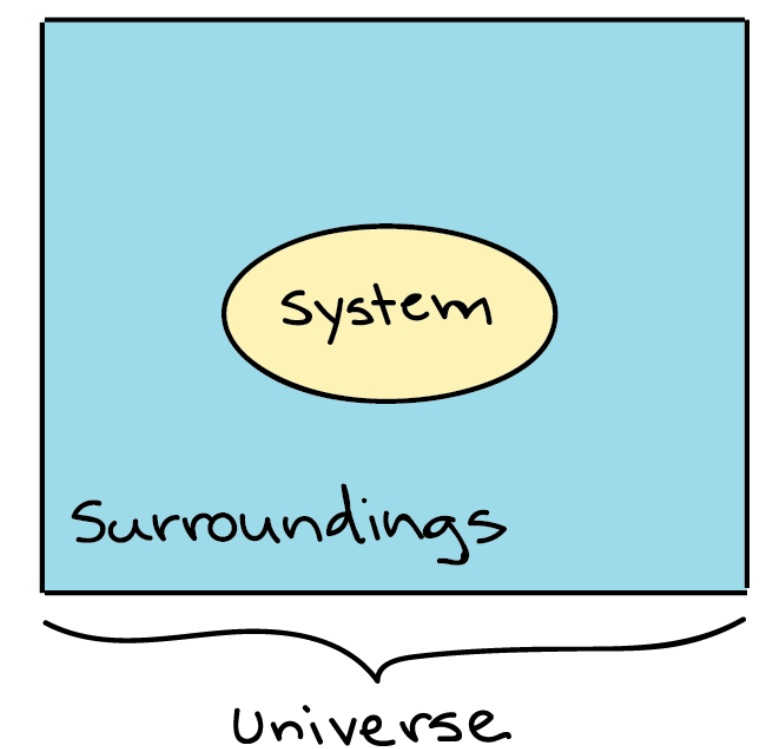
\includegraphics[width=0.4\textwidth]{figures/syst}
	\caption{The definition of a system and its surroundings in thermodynamics.}
	\label{fig:syst}
\end{figure}
The system and the surroundings together make up the universe. In general there are three categorizations of systems in thermodynamics:
\begin{enumerate}
	\item \emph{Open:} An open system is defined as a system that can exchange both energy and matter with its surroundings.
	
	\item \emph{Closed:} A closed system can exchange neither energy nor matter with its surroundings.
	
	\item \emph{Isolated:} An isolated system  can exchange either energy or matter with its surroundings.
\end{enumerate}
The system is said to be in thermodynamic equilibrium if the macroscopic variables characterizing the system (eg. $T,P,V,\dots$ of a gas) is independent of time. Central to thermodynamics is the notion of functions of state, the four laws to thermodynamics and the analysis of system stability.

\section{Functions of state}
As mentioned, a system is in thermodynamic equilibrium if the macroscopic observables are independent of time. The macroscopic observables are functions of state. A function of state is defined as the negative gradient of some abstract, conservative vector field(just like the case of equation \eqref{w6}). That is, a function of state is defined from the path integral
\begin{equation}
	\int_{\vec{x}_i}^{\vec{x}_f}df=f(\vec{x}_f)-f(\vec{x}_i).
	\label{f2}
\end{equation} 
The force field corresponding to the potential function is usually not ascribed any physical interpretation, it is the potential that has physical significance in this case - Since the potential is the physical observable. In general the differential of a function of state is called an exact differential. 
\begin{example}
	A conservative vector field has many useful properties, one of which is that the curl of the vector field is 0. This translates to symmetry of the second derivatives of the potential function. Eg. for a potential $U=U(S,V)$
	\begin{equation}
		\frac{\partial^2U}{\partial S\partial V}=\frac{\partial ^2U}{\partial V\partial S},
	\end{equation} 
	where $S,V$ at this point can be considered as nothing more than variables. Later on they can be considered as entropy($S$) and volume($V$). In thermodynamics, such relations are called Maxwell relations and will prove very useful when the potentials are expressed in terms of state functions.
\end{example}

\section{The laws of thermodynamics}
There are three principal laws of thermodynamics, however, these are supplemented by what is called the zeroth law of thermodynamics to make up four laws in total. Each law leads to the definition of thermodynamic properties which enables one to understand and predict the operation of a physical system.

\begin{enumerate}
	\item \emph{The zeroth law:} The zeroth law of thermodynamics state that two systems, each separately in thermal equilibrium with a third, are in equilibrium with each other. 
	
	\item \emph{The first law:} The first law of thermodynamics state that energy is conserved and heat and work are both forms of energy. The energy under consideration in thermodynamics is the internal energy, $U$. The internal energy is the sum of all the energy of all the internal degrees of freedom that the system posses. It is a function of state since the energy of a system is independent of how the energy is acquired. The internal energy of a system can be changed by doing work on the system or by being heated. The heat, $Q$, and work, $W$, are not functions of state since they describe how energy is delivered to the system. The equation describing the differential change in internal energy is the equation associated to the first law of thermodynamics
	\begin{equation}
		dU=\dbar Q+\dbar W,
	\end{equation} 
	where the bar-notation denotes inexact differentials. $\dbar Q>0$ is the heat applied to the system and $\dbar W>0$ is the work done on the system. $\dbar Q>0$.
	
	\item \emph{The second law:} The second law of thermodynamics can be formulated as a statement about the direction of heat flow that occurs as the system approaches equilibrium from an out of equilibrium state; no process is possible whose sole result is the transfer of heat from a colder to a hotter body. The most common manifestation of the second law of thermodynamics is in terms of entropy. Entropy in again defined in terms of the heat change under a reversible process. A reversible process is a process in which the system and surroundings can be restored to the initial state from the final state without producing any changes in the thermodynamic variables of the universe. In practice most processes are reversible\footnote{The macroscopic variables(eg. T, V,P) are only defined in equilibrium, so a quasi-static process has the macroscopic variables defined all the time - Unlike a process which is not quasi-static by fast.} if they are made sufficiently slow (quasi-static) such that the system passes through a series of equilibrium states between two macro-states. Any reversible process is quasi-static, but not all quasi-static processes are reversible. For example, a quasi-static process involving friction in the mechanics will not be reversible. In general are processes which involve a heat transfer between two systems not reversible. The change of entropy ($dS$) is defined in terms of the reversible change of heat $\dbar Q_{rev}$ as follows
	\begin{equation}
		dS=\frac{\dbar Q_{rev}}{T}.
	\end{equation} 
	The entropy is a state function so the differential is exact. Therefore, taking the endpoint to equal the initial point
	\begin{equation}
		\oint dS=\oint \frac{\dbar Q_{rev}}{T}=0.
		\label{ss1}
	\end{equation} 
	From Clausius theorem, for a process containing irreversible parts~\citep{blundell}
	\begin{equation}
		\oint \frac{\dbar Q}{T}\leq 0.
		\label{q1}
	\end{equation} 
	Taking $a\Rightarrow b$ to be done irreversibly and $b\Rightarrow a$ to be done reversible
	\begin{equation}
		\int_{a}^{b}\frac{\dbar Q}{T}+\int_{b}^{a}\frac{\dbar Q_{rev}}{T}\leq 0\Rightarrow \int_a^b\frac{\dbar Q}{T}\leq \int_{a}^{b}\frac{\dbar Q_{rev}}{T}.
		\label{q2}
	\end{equation} 
	Equation \eqref{q2} holds true however close $a,b$ are as points in state space. So, in general
	\begin{equation}
		dS=\frac{\dbar Q_{rev}}{T}\geq \frac{dQ}{T}.
		\label{q3}
	\end{equation} 
	The equality in $\geq$ only holds if the process is reversible. For an isolated system $\dbar Q=0$, so in general
	\begin{equation}
		dS\geq 0.
		\label{q4}
	\end{equation} 
	Equation \eqref{q4} states that any change for a thermally isolated system results in the entropy staying the same (for a reversible process) or increasing (for an irreversible process). This leads to another statement of the second law of thermodynamics; the entropy of an isolated system tends to a maximum. Equation \eqref{q4} is the manifestation of this version of the second law and is often used in analyzing the stability of thermodynamic systems. This version of the second law is also often applied to the universe. Taking th entire universe to be a closed system, it is clear that the entropy of the universe can only stay the same or go up\footnote{This description is on average. In analyzing the movement of individual molecules the entropy can indeed be found to go down.}. Taking $\dbar Q_{rev}=TdS$ and $\dbar W=-pdV+\mu dN+\dots$, where $p$ is pressure, $V$ is volume, $\mu$ is chemical potential and $N$ is the number of particles, the first law can be written viz
	\begin{equation}
		dU=TdS-pdV+\mu dN+\dots|_{rev}.
		\label{q5}
	\end{equation} 
	Equation \eqref{q5} is valid for reversible processes only at first glance. However, since all quantities in equation \eqref{q5} are functions of state (exact differentials), and therefore independent of the path in state space, the equation holds for irreversible processes as well. In irreversible processes $\dbar Q<0$ and $\dbar W>0$ such that $dU$ is the same whether the change is reversible or not. Hence, in general
	\begin{equation}
		dU=TdS-pdV+\mu dN+\dots.
		\label{q6}
	\end{equation} 
	
	\item \emph{The third law:} The third law of thermodynamics state that the entropy of all systems in internal equilibrium is the same at $T=0K$ (at absolute zero Kelvin), and may be taken to be zero, i.e.; $S(T=0K)=0$.
	
\end{enumerate} 

\section{Manipulation of thermodynamic potentials}	
A central part of practical application of thermodynamics is consist of manipulation of the thermodynamic potentials at hand. From the first law of thermodynamics
\begin{equation}
	dU=TdS-pdV+\mu dN+\dots.
	\label{qq1}
\end{equation} 
Note that $U=U(S,V,N,\dots)$. The potential $U$ can be transformed to another potential function, which is a function of different state functions, by performing a Legendre transformation(just as in advanced classical mechanics). The potential $U=U(S,V,N,\dots)$ can be transformed to the potential $F(T,V,N,\dots)$ viz
\begin{equation}
	\begin{split}
		dU&=TdS-pdV+\mu dN\dots\\
		&=d(TS)-SdT-pdV+\mu dN\dots.\\
	\end{split}
	\label{q12}
\end{equation} 
Taking $d(TS)$ to the left hand side of equation \eqref{q12} reveals
\begin{equation}
	\begin{split}
		dF(T,V,N,\dots)&=d(U(S,V,N,\dots)-TS)\\
		&=-SdT-pdV+\mu dN\dots.
	\end{split}
\end{equation} 
From the thermodynamic potentials, the equations of state are defied as the partial derivatives. From equation \eqref{q12}
\begin{equation}
	T=\frac{\partial U}{\partial S}\bigg|_{V,N,\dots}, \quad -p=\frac{\partial U}{\partial V}\bigg|_{S,N,\dots}, \quad \mu=\frac{\partial U}{\partial N}\bigg|_{S,V,\dots}, \quad \dots.
	\label{q7}
\end{equation} 
Similar equations of state can be derived from $F$. The equation of equation \eqref{q7} are called equations of state. Equations of state are the first partial derivatives of thermodynamic potentials. Now, from the Maxwell relations
\begin{equation}
	\begin{split}
		&\frac{\partial^2 U}{\partial S\partial V}=\frac{\partial^2 U}{\partial V\partial S}\Rightarrow -\frac{\partial p}{\partial S}\bigg|_{_{N,\dots}}=\frac{\partial T}{\partial V}\bigg|_{_{N,\dots}},\\
		&\frac{\partial^2 U}{\partial N\partial V}=\frac{\partial^2 U}{\partial V\partial N}\Rightarrow -\frac{\partial p}{\partial N}\bigg|_{_{S,\dots}}=\frac{\partial \mu}{\partial V}\bigg|_{_{S,\dots}},\\
		&\frac{\partial^2 U}{\partial N\partial S}=\frac{\partial^2 U}{\partial S\partial N}\Rightarrow \frac{\partial T}{\partial N}\bigg|_{_{V,\dots}}=\frac{\partial \mu}{\partial S}\bigg|_{_{V,\dots}}.\\
	\end{split}
	\label{q8}
\end{equation} 
The Maxwell relations are often supplemented by mathematical tools such as Eulers triangle rule and the reciprocal theorem. Eulers triangle rule
\begin{equation}
	\text{Eulers triangle rule:} \quad \frac{\partial S}{\partial T}\bigg|_{_{V,N,\dots}}\frac{\partial T}{\partial V}\bigg|_{_{S,N,\dots}}\frac{\partial V}{\partial S}\bigg|_{_{T,N,\dots}}=-1.
	\label{q9}
\end{equation} 
Note how the derivatives are cyclic, and the relation can be composed from just \textbf{one} partial derivative. The reciprocal theorem
\begin{equation}
	\text{Reciprocal tehorem:}\quad \Rightarrow \frac{\partial S}{\partial V}\bigg|_{_{T,N,\dots}}=\frac{1}{\frac{\partial V}{\partial S}\big|_{_{T,N,\dots}}}.
	\label{q10}    
\end{equation} 

\begin{example}
	Eulers triangle rule and the reciprocal theorem are often used in conjunction to rewrite state functions viz
	\begin{equation}
		\frac{\partial S}{\partial T}\bigg|_{_{V,N,\dots}}=-\frac{\partial S}{\partial V}\bigg|_{_{T,N,\dots}}\frac{\partial V}{\partial T}\bigg|_{_{S,N,\dots}}  .
	\end{equation}  
	In this way, a possibly non-calculable differential can be turned into a perhaps calculate-able one. These relations can in turn be combined with the equations of state and the Maxwell relations in order to really make the magic happen. 
\end{example}

\section{System stability}
In thermodynamics the thermodynamic potentials are often used to analyze the stability of the system. The condition for stability is that for fixed variables, any change in the thermodynamic potential system must be positive. For example for $F=F(T,V,N)$ when $T,V,N$ are fixed, $\delta F \geq0$. Another way of stating this is that if you leave a system alone, it is stable if it is in a minimum of the potential. In the minimum, every change in the potential is positive! In equilibrium, the potential must be convex. A convex function has a positive curvature. This is mathematically expressed as
\begin{equation}
	d^2F>0
\end{equation}   
To examine the stability, investigate the fluctuations between two subsystems, when the system is in a stable equilibrium. Take $N=const$, while allowing $T,V$ to vary. A small perturbation in the potential can then be written as follows
\begin{equation}
	\delta F=F_2(T+\Delta T, V+\Delta V, N)+F_1(T-\Delta T, V- \Delta V, N) - 2F(T,M,N)\geq 0,
	\label{variationF}
\end{equation} 
where the last term is included to subtract the average offset of the potential. Only the fluctuations around the minimum is of interest, not with respect to the arbitrary reference value that has been chosen. Next, Taylor expand $F_1 $ and $F_2$
\begin{equation}
	\begin{split}
		&F_2=F(T,V,N)+\frac{\partial F}{\partial T}\bigg|_{_{V,N}}\Delta T+\frac{\partial F}{\partial V}\bigg|_{_{T,N}}\Delta V\\
		&\qquad+\frac{1}{2}\bigg(\frac{\partial^2 F}{\partial T^2}\bigg|_{_{V,N}}(\Delta T)^2+\frac{\partial^2 F}{\partial V^2}\bigg|_{_{T,N}}(\Delta V)^2+2\frac{\partial^2 F}{\partial T \partial V}\bigg|_{_{N}}\Delta M \Delta T \bigg)+...,\\
		&F_1=F(T,V,N)-\frac{\partial F}{\partial T}\bigg|_{_{V,N}}\Delta T-\frac{\partial F}{\partial V}\bigg|_{_{T,N}}\Delta V\\
		&\qquad+\frac{1}{2}\bigg(\frac{\partial^2 F}{\partial T^2}\bigg|_{_{V,N}}(\Delta T)^2 +\frac{\partial^2 F}{\partial V^2}\bigg|_{_{T,N}}(\Delta V)^2+2\frac{\partial^2 F}{\partial T \partial V}\bigg|_{_{N}}\Delta V \Delta T \bigg)+...,
	\end{split}
	\label{taylor}
\end{equation}  
where the terms of higher order is neglected in the usual analysis of stability. By inserting equation \eqref{taylor} in equation \eqref{variationF}, the first order terms, along with the zero order terms, disappear and leave only the second order terms. Let the changes go to infinitesimal sizes ($\Delta \Rightarrow d$) to find
\begin{equation}
	\delta F\cong\frac{\partial^2 F}{\partial T^2}\bigg|_{_{V,N}}(dT)^2+\frac{\partial^2 F}{\partial V^2}\bigg|_{_{T,N}}(dV)^2+2\frac{\partial^2 F}{\partial T \partial V}\bigg|_{_{N}}dVdT=d^2F > 0.
	\label{d^2F}
\end{equation} 
The "$\cong$" in equation \eqref{d^2F} come from neglecting higher order terms from the Taylor series. Equation \eqref{d^2F} can be written in matrix form
\begin{equation}
	d^2F=
	\begin{bmatrix}
		dT & dV\\
	\end{bmatrix}
	\begin{bmatrix}
		\frac{\partial^2 F}{\partial T^2}\bigg|_{_{V,N}}       & \frac{\partial^2 F}{\partial T \partial V}\bigg|_{_{N}}  \\
		\frac{\partial^2 F}{\partial T \partial V}\bigg|_{_{N}}       &
		\frac{\partial^2 F}{\partial V^2}\bigg|_{_{T,N}}
		\\
	\end{bmatrix}
	\begin{bmatrix}
		dT\\
		dV\\
	\end{bmatrix} > 0.
	\label{matrix1}
\end{equation} 
Since the matrix is symmetric, it can be diagonalized with the eigenvalues in the diagonal. That is, equation \eqref{matrix1} can be written on the form
\begin{equation}
	d^2F=
	\begin{bmatrix}
		dT & dV\\
	\end{bmatrix}
	\begin{bmatrix}
		\lambda_1       & 0  \\
		0       &
		\lambda_2
		\\
	\end{bmatrix}
	\begin{bmatrix}
		dT\\
		dM\\
	\end{bmatrix}=\lambda_1(dT)^2+\lambda_2(dV)^2 > 0.
\end{equation} 
For this expression to hold for every possible eigenvalue, the eigenvalues must be positive. Since they must be positive, the determinant and trace of the diagonalized matrix must be positive as well. That is
\begin{equation}
	\begin{split}
		det
		\begin{bmatrix}
			\lambda_1       & 0  \\
			0       &
			\lambda_2
			\\
		\end{bmatrix}&=\lambda_1 \lambda_2 >0,\\
		tr
		\begin{bmatrix}
			\lambda_1       & 0  \\
			0       &
			\lambda_2
			\\
		\end{bmatrix}&=\lambda_1 + \lambda_2 >0.
	\end{split}
\end{equation} 
Note that the determinant can be positive if both eigenvalues are negative, and the trace can be positive if the smallest eigenvalue is negative. If both conditions are fulfilled, then both eigenvalues must be positive. A diagonalization is a linear transformation. Under such a transformation both the determinant and trace are conserved quantities. That means the trace and determinant of the diagonalized matrix can be determined directly from the undiagonalized matrix. No diagonalization have to be performed in practice. The determinant and trace of the "middle" matrix in equation \ref{matrix1}, are in this case found to be:
\begin{equation}
	\begin{split}
		det
		\begin{bmatrix}
			\frac{\partial^2 F}{\partial T^2}\bigg|_{_{V,N}}       & \frac{\partial^2 F}{\partial T \partial V}\bigg|_{_{N}}  \\
			\frac{\partial^2 F}{\partial T \partial V}\bigg|_{_{N}}       &
			\frac{\partial^2 F}{\partial V^2}\bigg|_{_{T,N}}
			\\
		\end{bmatrix}
		&=\frac{\partial^2 F}{\partial T^2}\bigg|_{_{V,N}}\frac{\partial^2 F}{\partial V^2}\bigg|_{_{T,N}}-\bigg(\frac{\partial^2 F}{\partial T \partial V}\bigg|_{_{N}}\bigg)^2 >0\\
		tr
		\begin{bmatrix}
			\frac{\partial^2 F}{\partial T^2}\bigg|_{_{V,N}}       & \frac{\partial^2 F}{\partial T \partial V}\bigg|_{_{N}}  \\
			\frac{\partial^2 F}{\partial T \partial V}\bigg|_{_{N}}       &
			\frac{\partial^2 F}{\partial V^2}\bigg|_{_{T,N}}
			\\
		\end{bmatrix}
		&=\frac{\partial^2 F}{\partial T^2}\bigg|_{_{V,N}}+\frac{\partial^2 F}{\partial V^2}\bigg|_{_{T,N}}>0
	\end{split}
	\label{det}
\end{equation} 
After this expression is reached, the expressions for the derivatives must be analyzed in order to interpret the physical content of the stability of the system \footnote{Note that \ref{det} is derived on the basis that a perturbation in V and T is performed whilst N is held constant. If these conditions are not met, the equations does not hold(!).}. The second derivatives couple to the heat capacities, so the stability of the system couples to the allowed signs of the heat capacities\footnote{Often they must be positive in a stable system}. Further more, the general derivatives can be analyzed by determining whether a thermodynamic variable is extensive or intensive. Thermodynamic potentials are convex functions of their extensive variables, and concave functions of their intensive variables. For example the temperature is an intensive variable; it does not change if the system size is altered. From this it can be concluded that $\frac{\partial^2 F}{\partial T^2}\big|_{_{M,N}}\leq0$. Likewise for other thermodynamic variables and potentials\footnote{That goes for the evaluation of the second derivatives as well as the stability treatment of the potential.}.